\section{Depósito Documental de Evidencias}
\label{sec:evidencias}

En esta sección se compilan las capturas de pantalla, respuestas de servidor, consultas HTTP (Postman) o logs del sistema para cada uno de los casos. 

\textbf{Indicaciones:} Por favor, asegúrese de adjuntar las evidencias en los espacios designados utilizando referencias relativas.

\subsection{Pruebas Funcionales}

\begin{itemize}
    \item \textbf{CP-F-01} (Registrar incidencia) - Fecha: 7/07/2026
    \begin{itemize}
        \item \textbf{Resultado:} [Aprobado]
        \item \textit{Evidencia:}
        
        \begin{figure}[H] % La 'H' mayúscula obliga a la imagen a quedarse EXACTAMENTE aquí
            \centering
            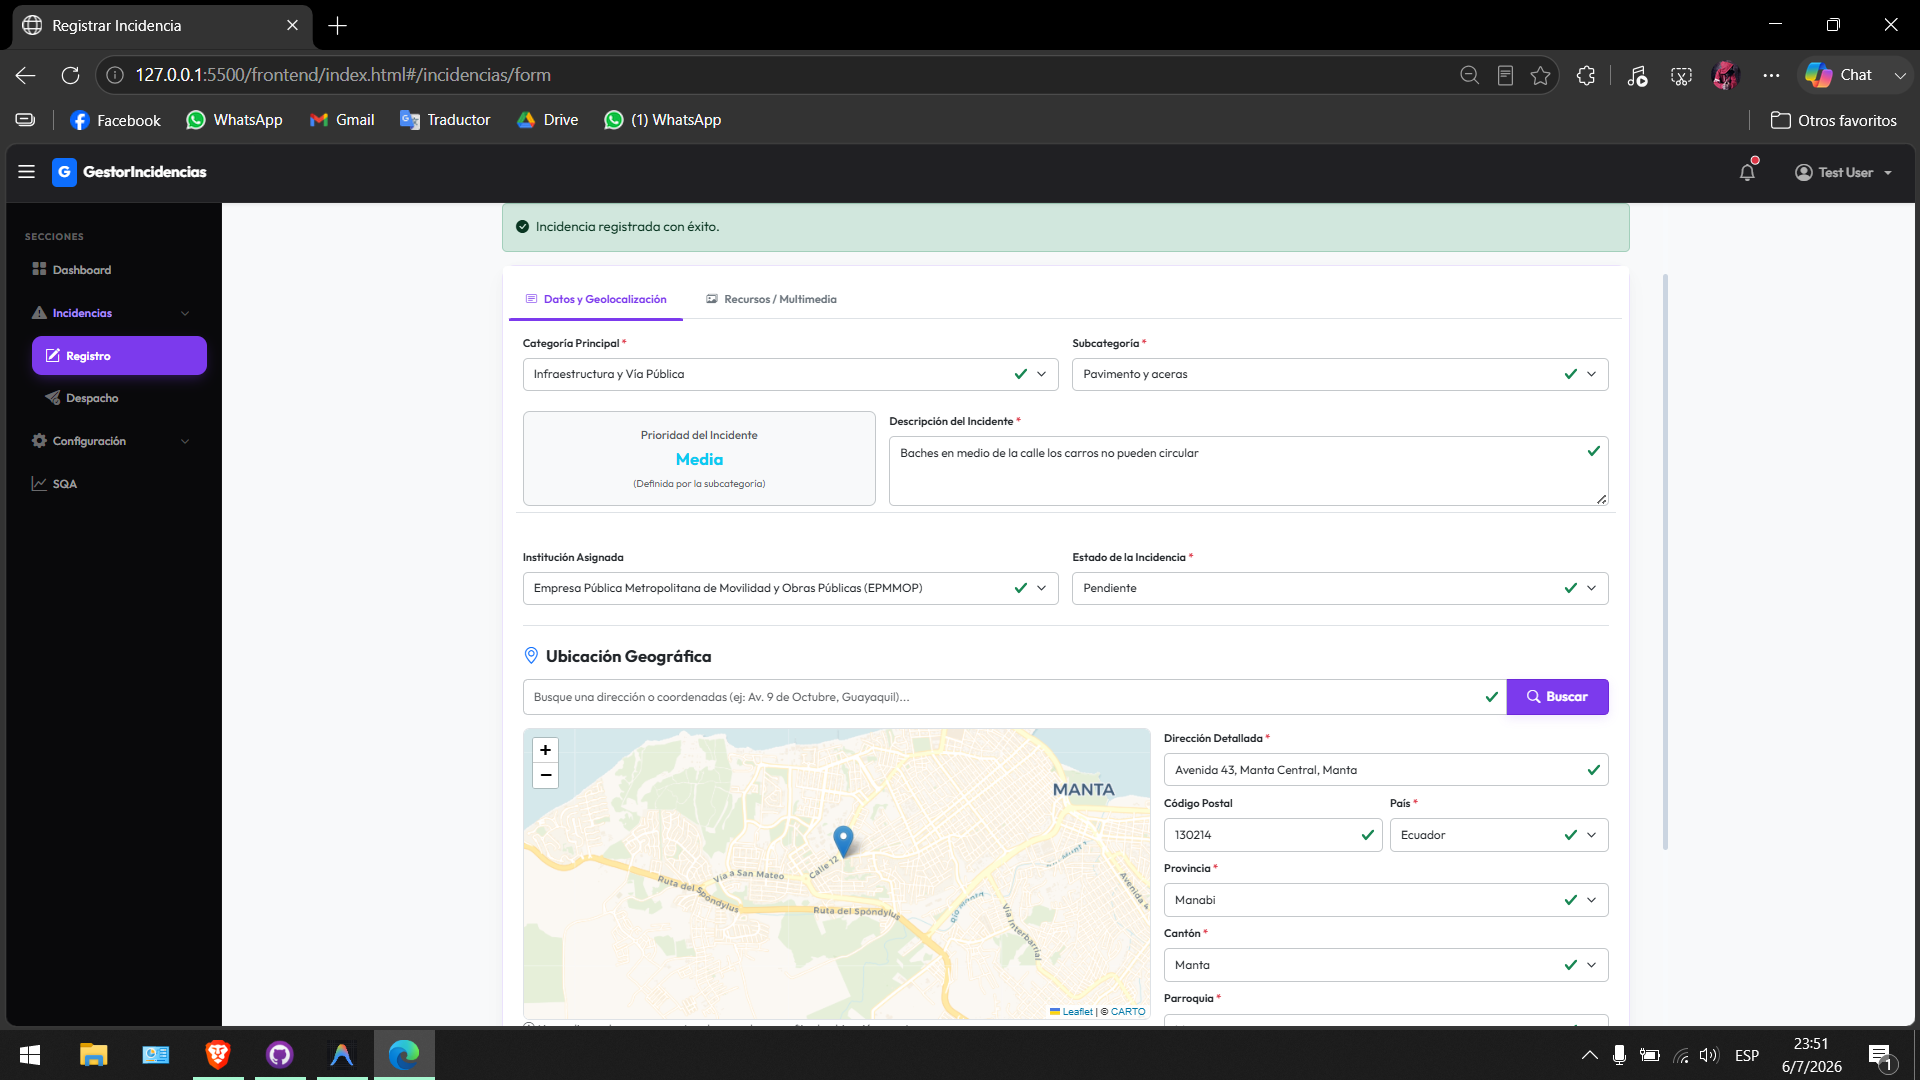
\includegraphics[width=0.9\textwidth]{imagenes/cp-f-01-exito.png}
            \caption{Evidencia.}
        \end{figure}
        El caso de éxito se presenta cuando se selecciona una ubicación en la
        que ya esté correctamente estandarizados su cantón y su parroquia.
        Pero no se tiene certeza de que cualquier punto del mapa tenga una parroquia.

        \begin{figure}[H] % La 'H' mayúscula obliga a la imagen a quedarse EXACTAMENTE aquí
            \centering
            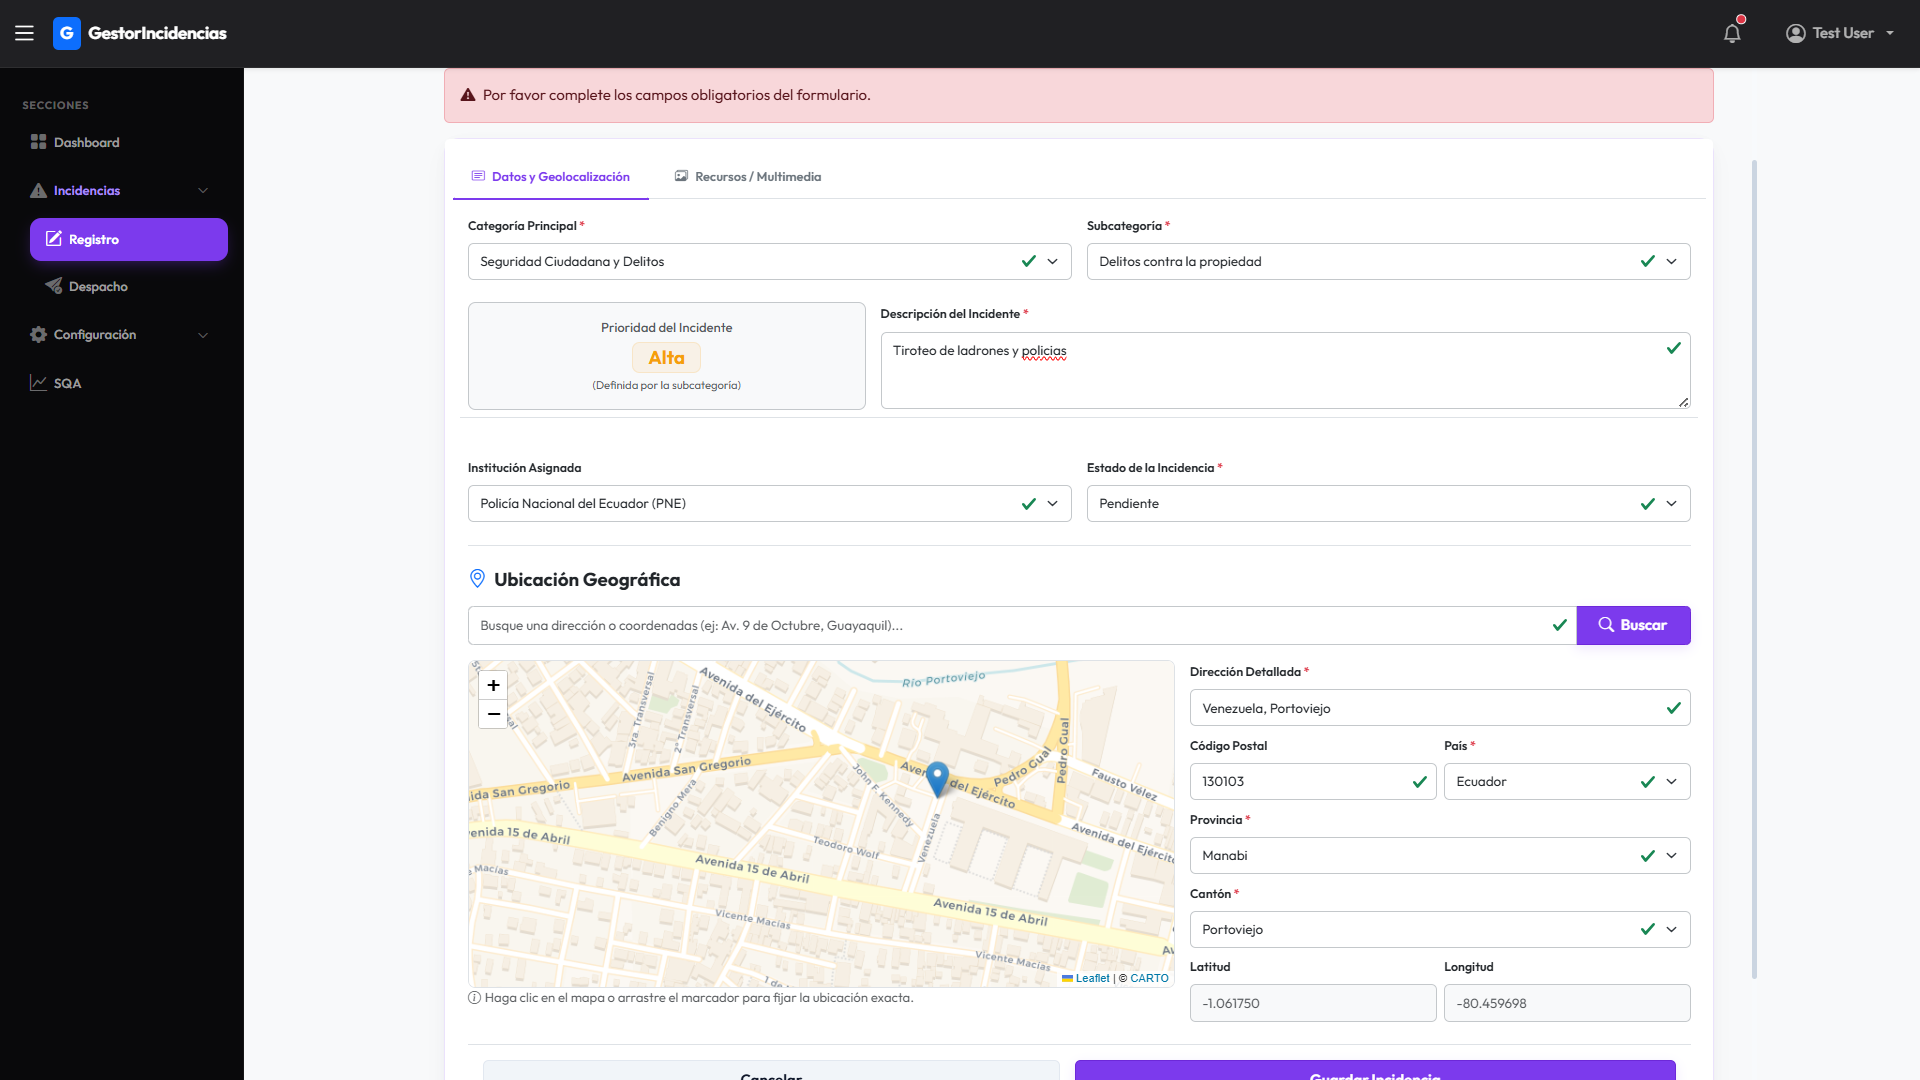
\includegraphics[width=0.9\textwidth]{imagenes/cp-f-01-fallo.png}
            \caption{Evidencia.}
        \end{figure}
        El caso de fracaso se da cuando Leaflet no encuentra la parroquia del cantón seleccionado.
        Esto se solucionará con un flag interno que indique cuándo el cantón seleccionado necesite especificar una parroquia.
        Y se le habilitará al usuario para que seleccione la ubicación en la que se encuentra.

        \begin{figure}[H] % La 'H' mayúscula obliga a la imagen a quedarse EXACTAMENTE aquí
            \centering
            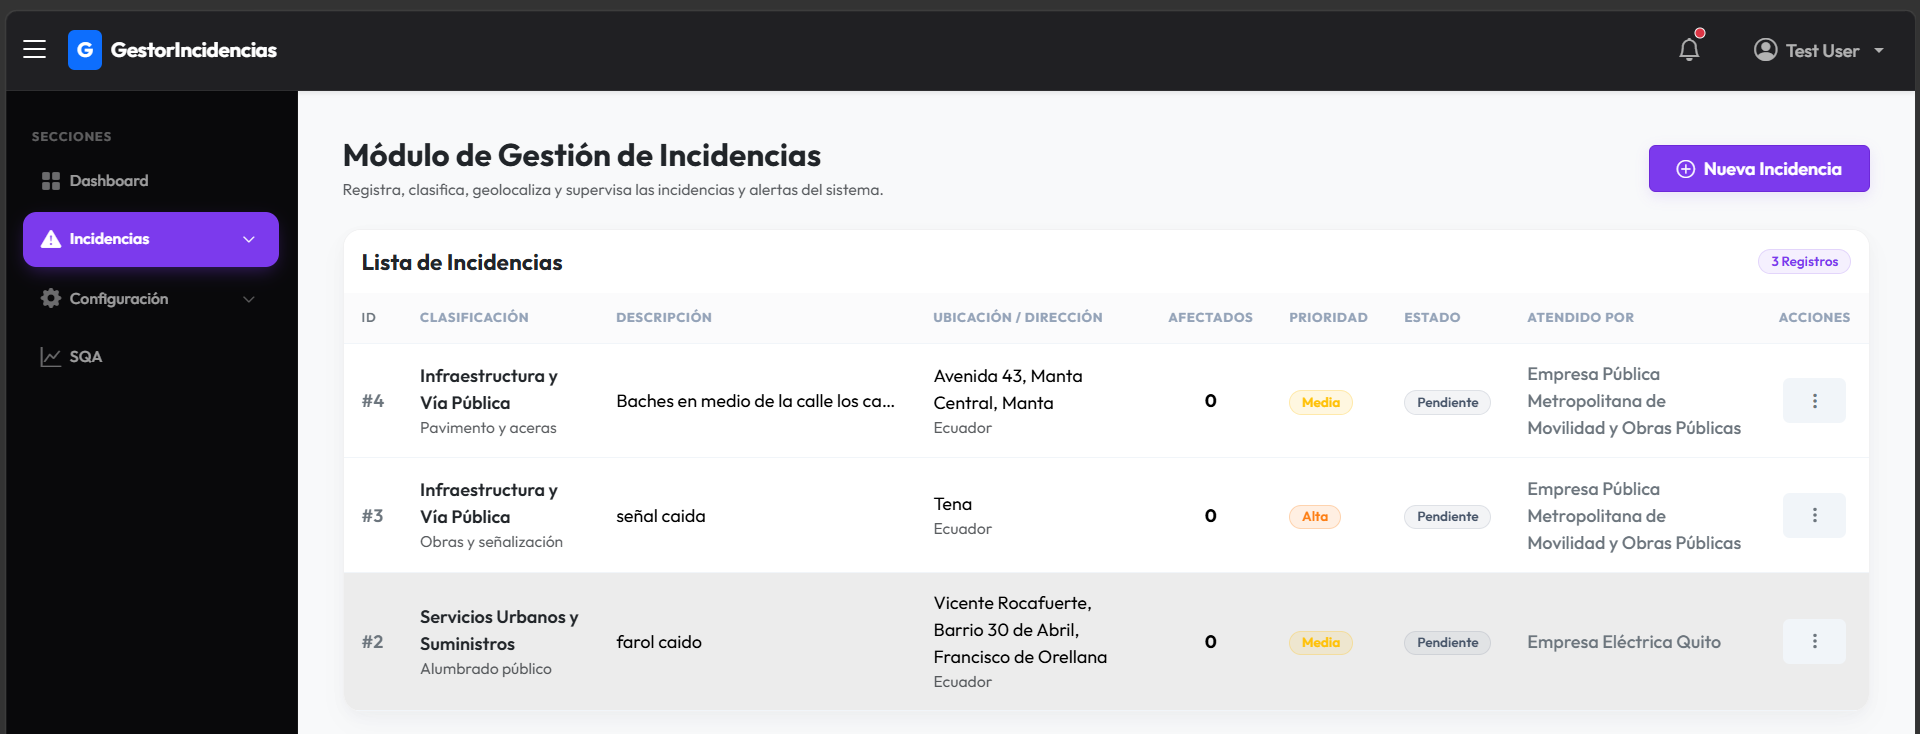
\includegraphics[width=0.9\textwidth]{imagenes/cp-f-01-lista.png}
            \caption{Evidencia.}
        \end{figure}
    \end{itemize}

    \item \textbf{CP-F-02} (Editar incidencia) - Fecha: 7/07/2026
    \begin{itemize}
        \item \textbf{Resultado:} [Aprobado]
        \item \textit{Evidencia:}
        
        \begin{figure}[H] % La 'H' mayúscula obliga a la imagen a quedarse EXACTAMENTE aquí
            \centering
            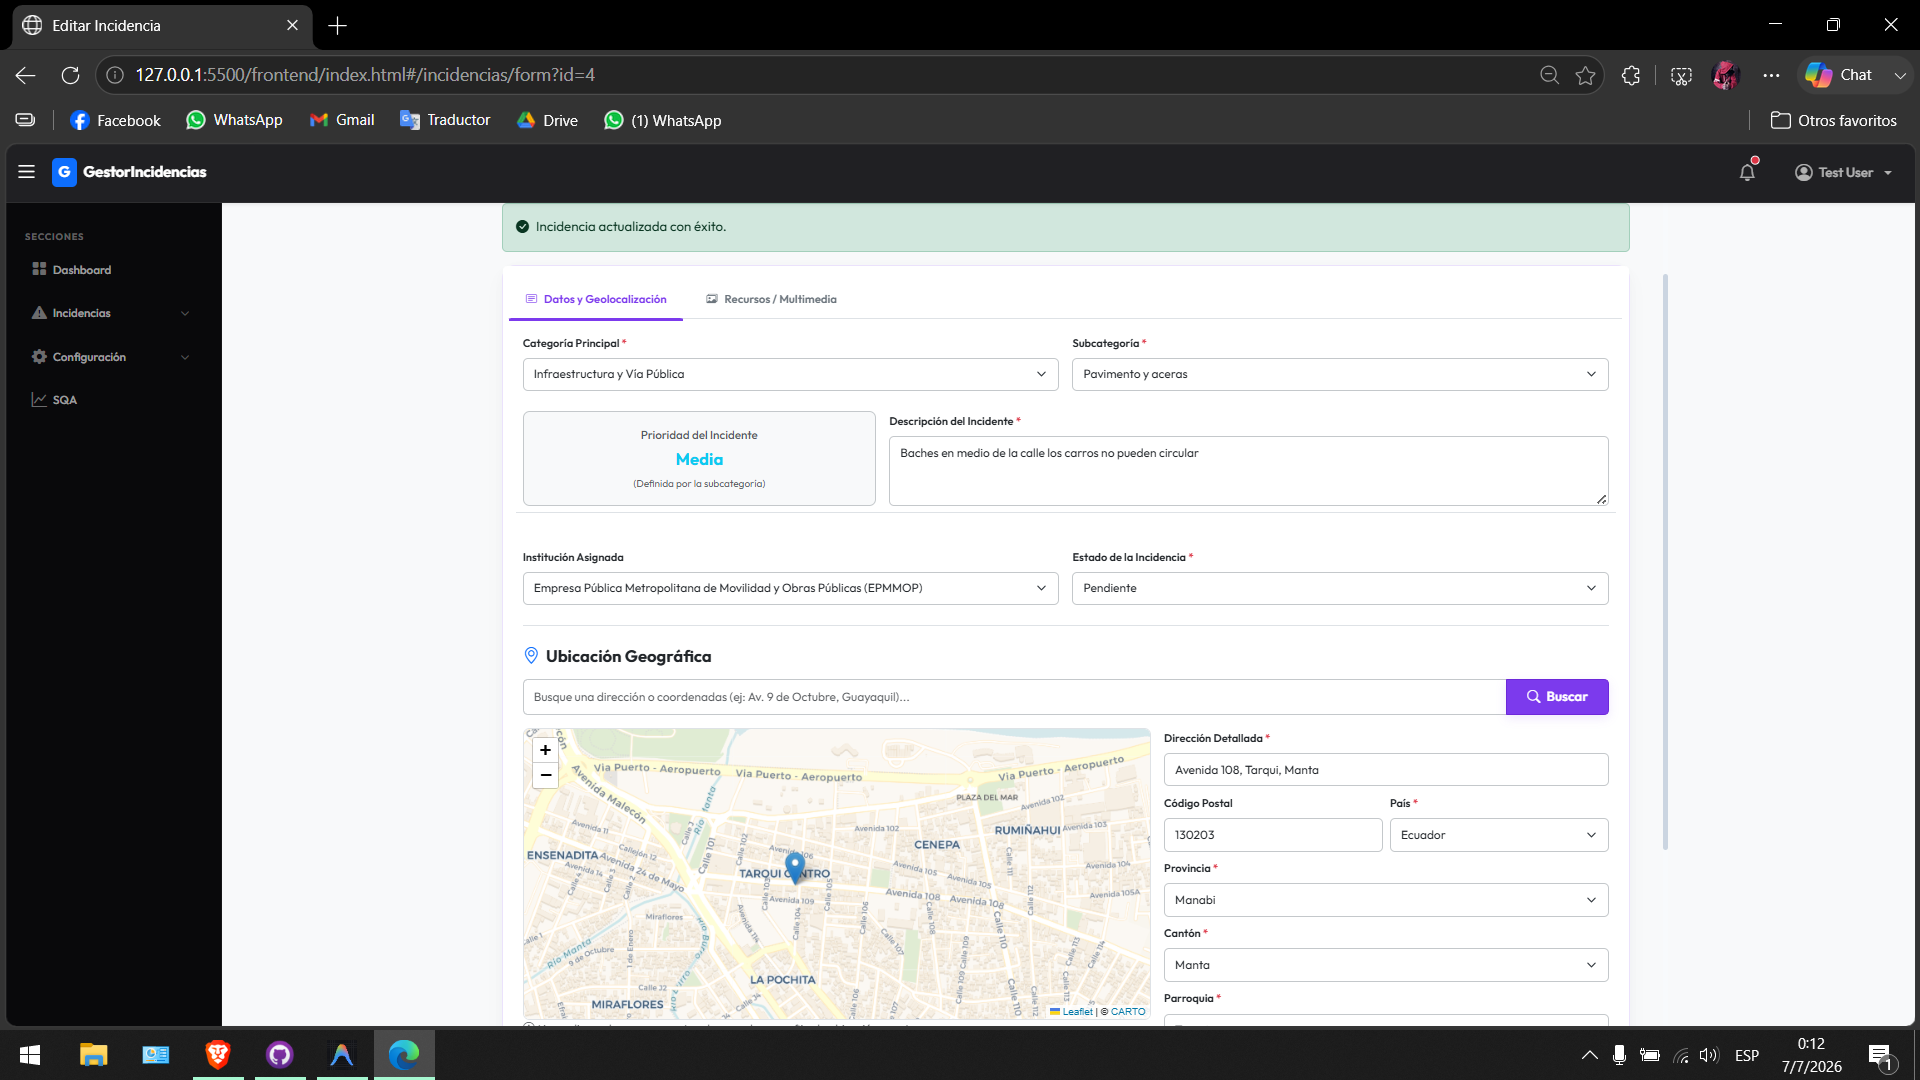
\includegraphics[width=0.9\textwidth]{imagenes/cp-f-02-exito.png}
            \caption{Evidencia.}
        \end{figure}
        Aqui cambiamos la parroquia de Manta a Tarqui.

    \end{itemize}
    \item \textbf{CP-F-03} (Eliminación lógica) - Fecha: 7/07/2026
    \begin{itemize}
        \item \textbf{Resultado:} [Aprobado]
        \item \textit{Evidencia:}
        
         \begin{figure}[H] % La 'H' mayúscula obliga a la imagen a quedarse EXACTAMENTE aquí
            \centering
            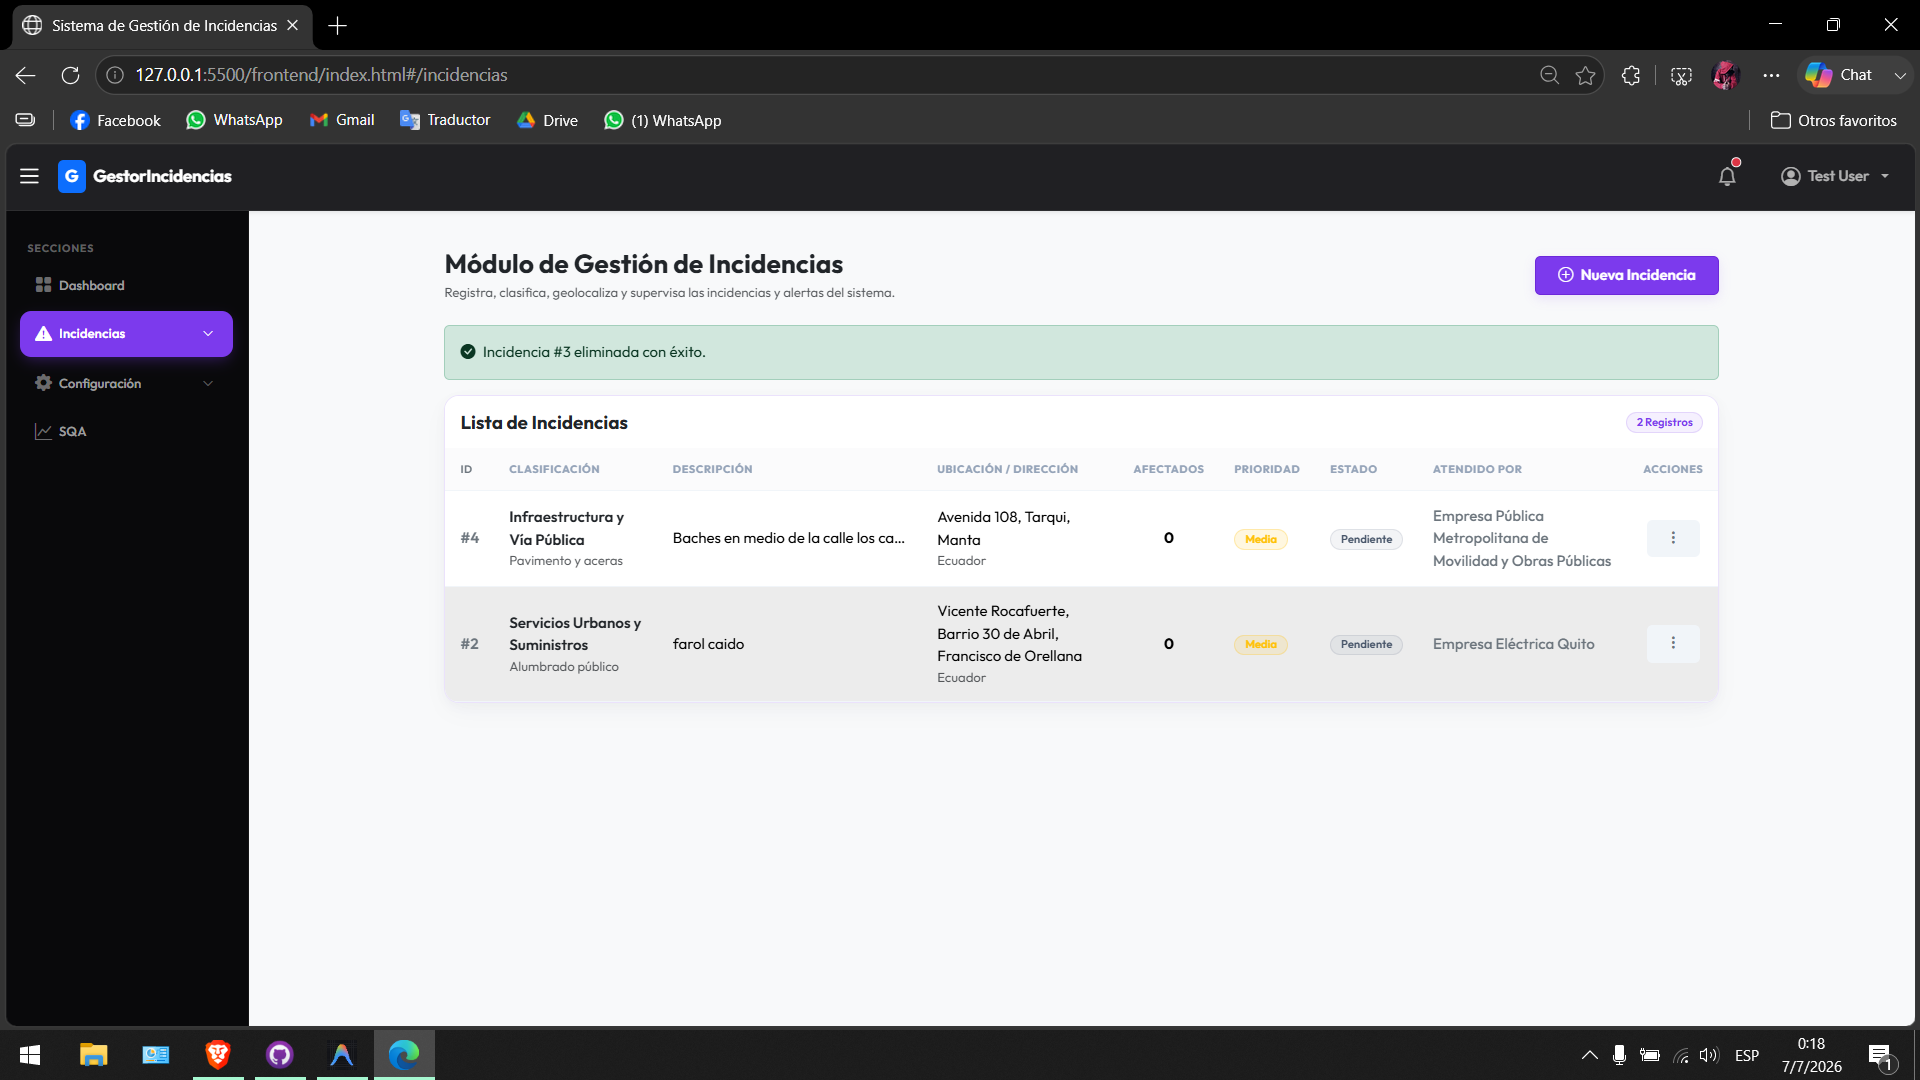
\includegraphics[width=0.9\textwidth]{imagenes/cp-f-03.png}
            \caption{Evidencia.}
        \end{figure}
        Aquí se elimina una incidencia de la tabla de incidencias. En la imagen se ven solo 2 registros.

        \begin{figure}[H] % La 'H' mayúscula obliga a la imagen a quedarse EXACTAMENTE aquí
            \centering
            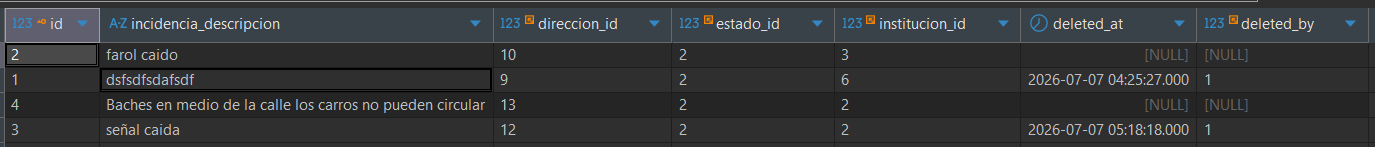
\includegraphics[width=0.9\textwidth]{imagenes/cp-f-03-soft.png}
            \caption{Evidencia.}
        \end{figure}
        Y en los datos reales comprobamos que no se han eliminado de la BD sino que se ha ejecutado un soft delete.
    \end{itemize}

    \item \textbf{CP-F-04} (Cambio de estado) - Fecha: 8/07/2026
    \begin{itemize}
        \item \textbf{Resultado:} [Aprobado]
        \item \textit{Evidencia:}
        
        \begin{figure}[H] % La 'H' mayúscula obliga a la imagen a quedarse EXACTAMENTE aquí
            \centering
            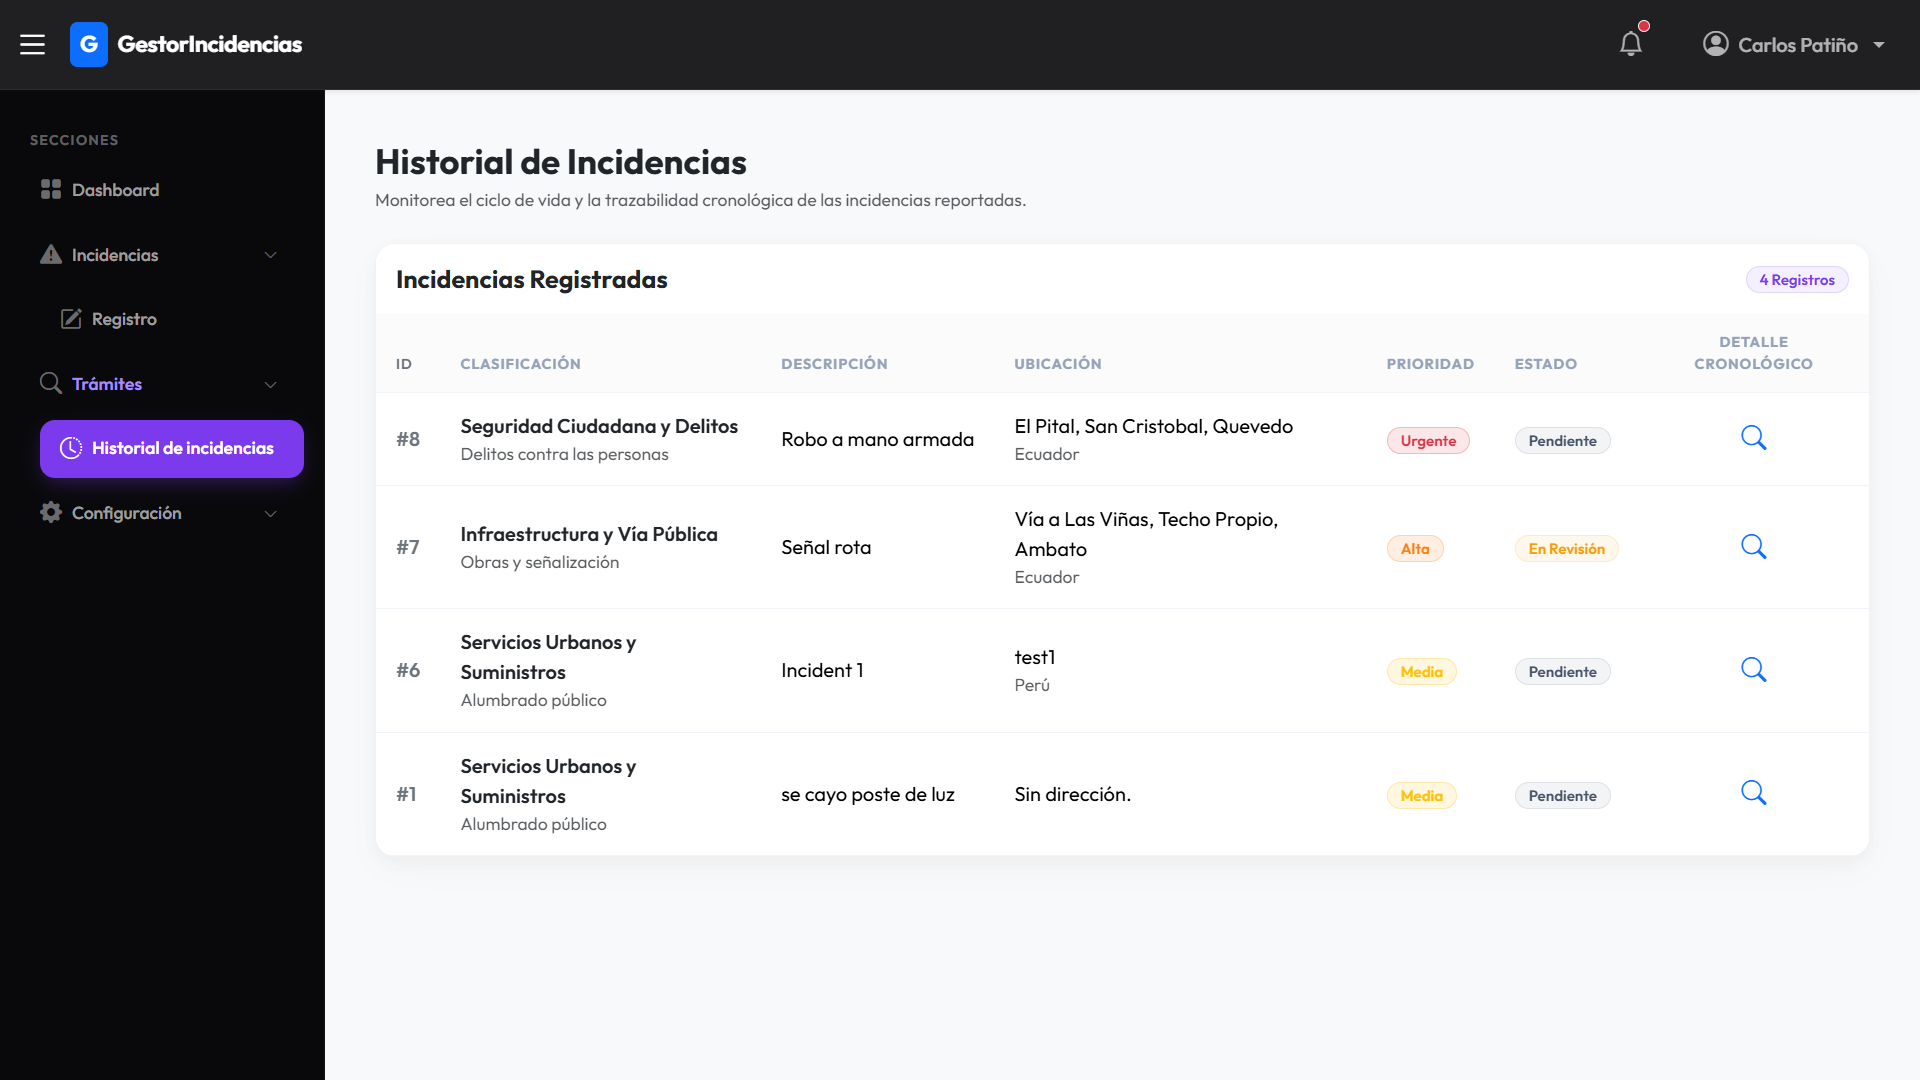
\includegraphics[width=0.9\textwidth]{imagenes/cp-f-04.png}
            \caption{Evidencia.}
        \end{figure}
        Al registrar una incidencia, el estado por defecto es pendiente. En la imagen se que la incidencia con descripción "Robo a mano armada" tiene su estado Pendiente, porque recién se ha creado.

        \begin{figure}[H] % La 'H' mayúscula obliga a la imagen a quedarse EXACTAMENTE aquí
            \centering
            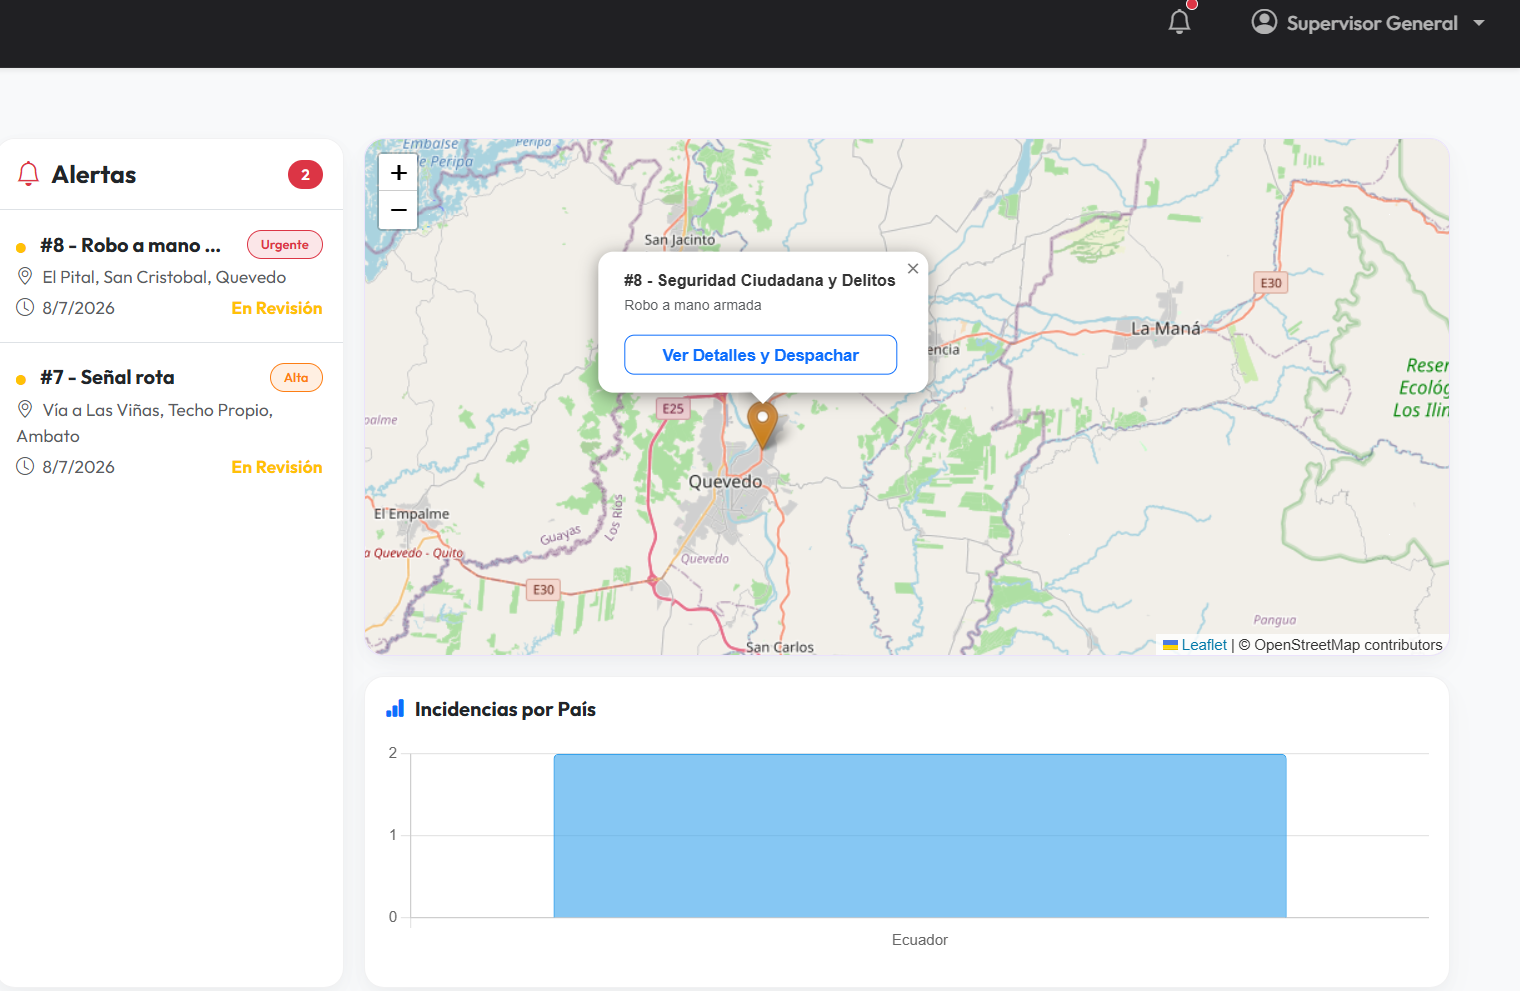
\includegraphics[width=0.9\textwidth]{imagenes/cp-f-04-despacho.png}
            \caption{Evidencia.}
        \end{figure}
        En esta imagen se ve la pantalla de despacho del Supervisor. Cuando el supervisor entra a la pantalla, el estado cambia a En revisión, indicando que están al tanto de la incidencia.

        \begin{figure}[H] % La 'H' mayúscula obliga a la imagen a quedarse EXACTAMENTE aquí
            \centering
            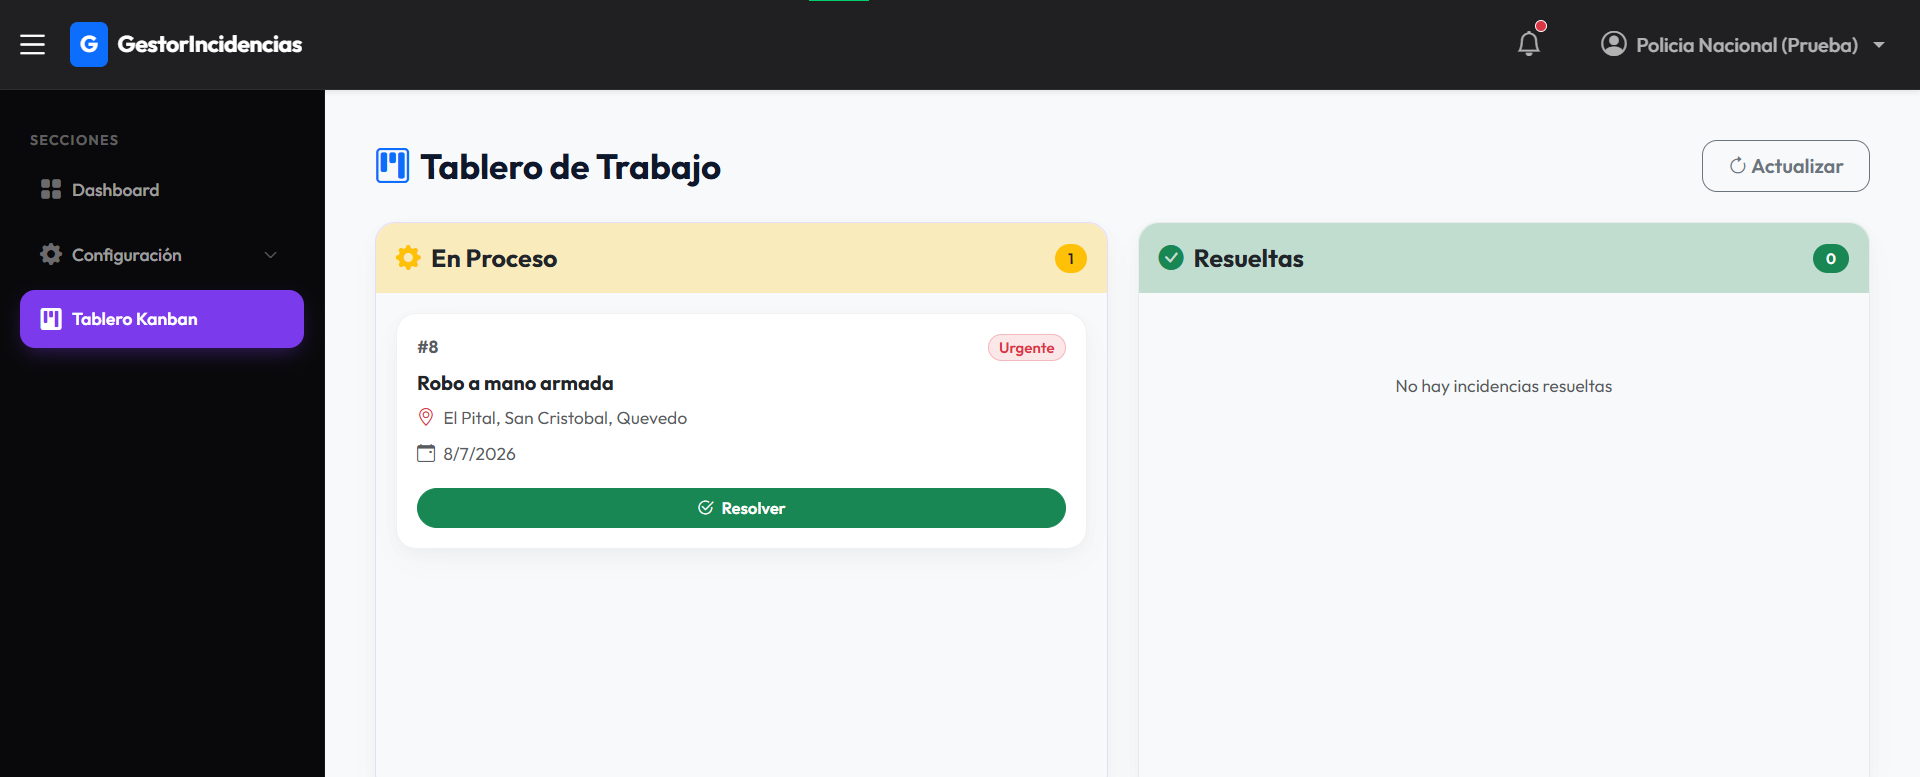
\includegraphics[width=0.9\textwidth]{imagenes/cp-f-04-kanban.png}
            \caption{Evidencia.}
        \end{figure}
        Cuando el supervisor despacha, el item desaparece, la incidencia pasa a estado "En proceso" y el rol de Insitución encargado estará al tanto en su tablero Kanban. Este es un WIP donde la institución tendrá que marcar como resuelta la incidencia.

        \begin{figure}[H] % La 'H' mayúscula obliga a la imagen a quedarse EXACTAMENTE aquí
            \centering
            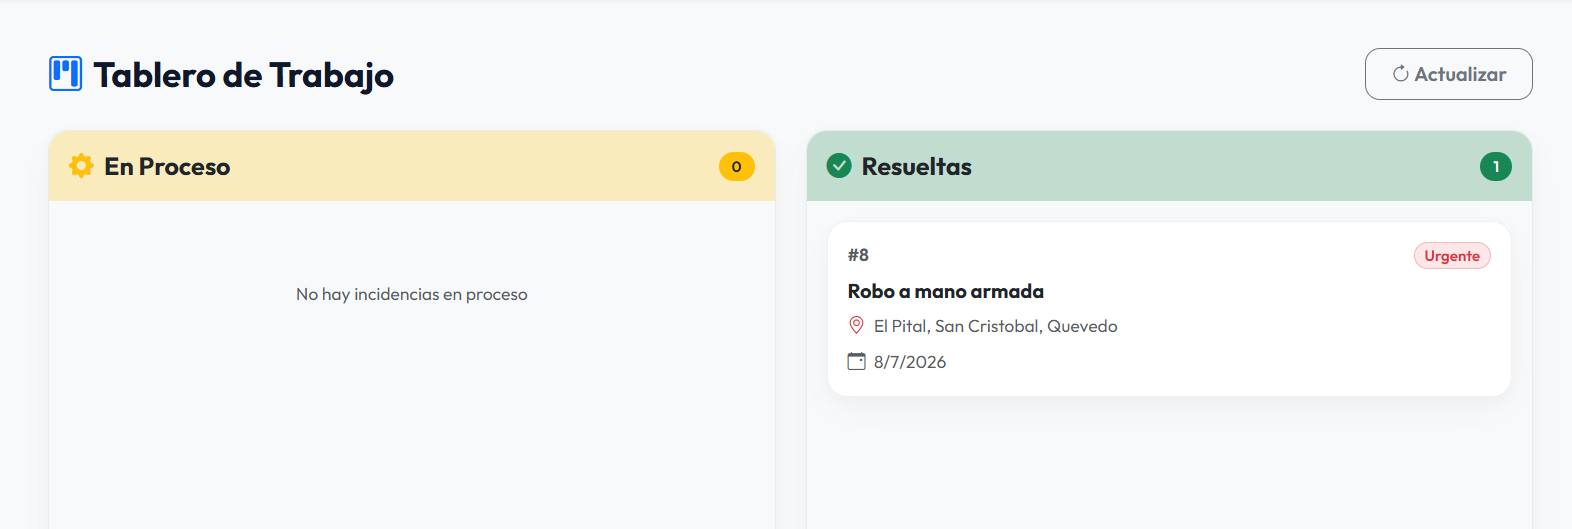
\includegraphics[width=0.9\textwidth]{imagenes/cp-f-04-resuelto.png}
            \caption{Evidencia.}
        \end{figure}
        El mismo rol de institución puede ver que el item pasa a estado resuelto, y el usuario podrá consultar su historial donde verá su incidencia como resuelta.

    \end{itemize}

    \item \textbf{CP-F-05} (Historial de cambios) - Fecha: 8/07/2026
    \begin{itemize}
        \item \textbf{Resultado:} [Aprobado]
        \item \textit{Evidencia:}
        
        \begin{figure}[H] % La 'H' mayúscula obliga a la imagen a quedarse EXACTAMENTE aquí
            \centering
            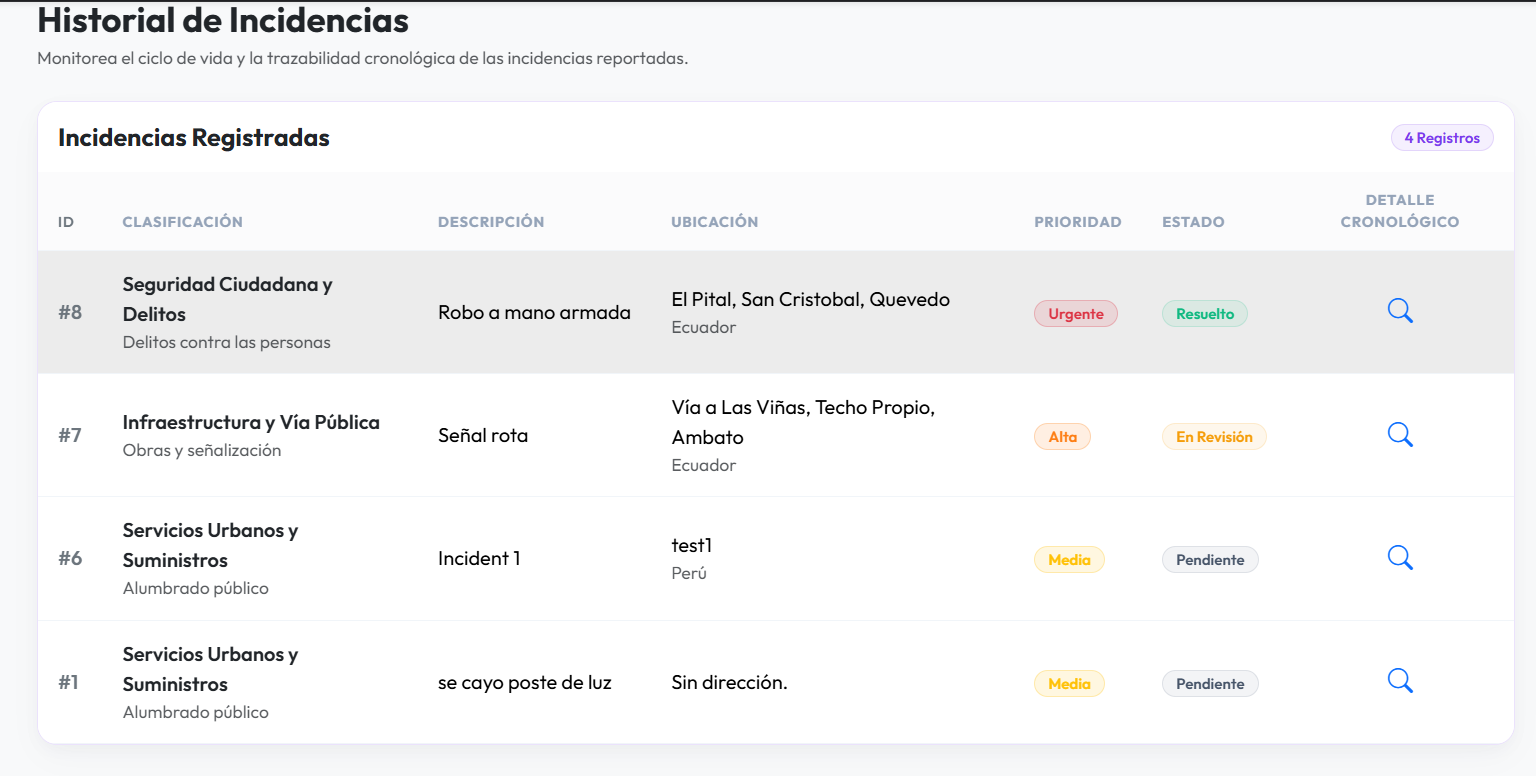
\includegraphics[width=0.9\textwidth]{imagenes/cp-f-05.png}
            \caption{Evidencia.}
        \end{figure}
    \end{itemize}

    \item \textbf{CP-F-06} (Asignar responsable) - Fecha: 7/07/2026
    \begin{itemize}
        \item \textbf{Resultado:} [Aprobado]
        \item \textit{Evidencia:}
        
        Los responsables están atados directamente a su subcategoría

        \begin{figure}[H] % La 'H' mayúscula obliga a la imagen a quedarse EXACTAMENTE aquí
            \centering
            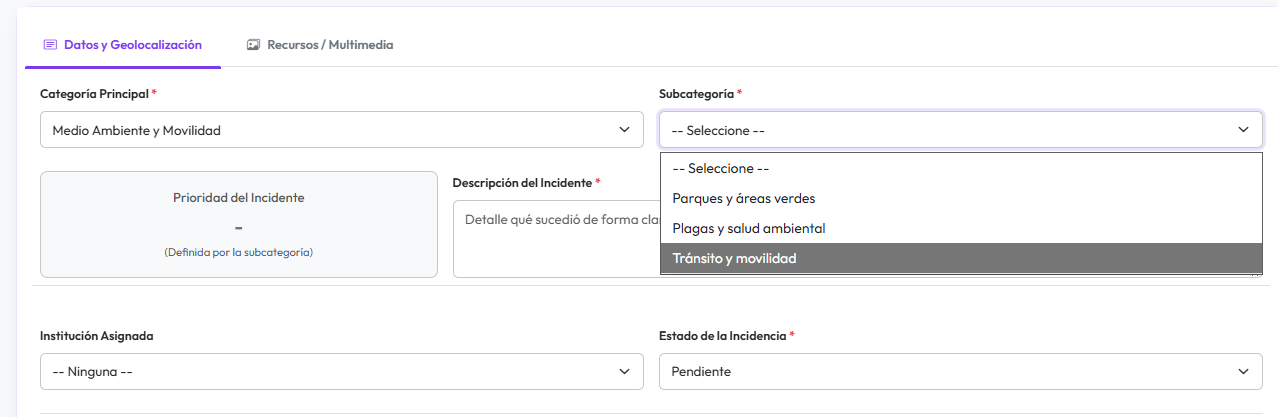
\includegraphics[width=0.9\textwidth]{imagenes/cp-f-06-asignar-subcat-primero.png}
            \caption{Evidencia.}
        \end{figure}
        Al elegir la subcategoría, se seleccionará el responsable pertinente.

        \begin{figure}[H] % La 'H' mayúscula obliga a la imagen a quedarse EXACTAMENTE aquí
            \centering
            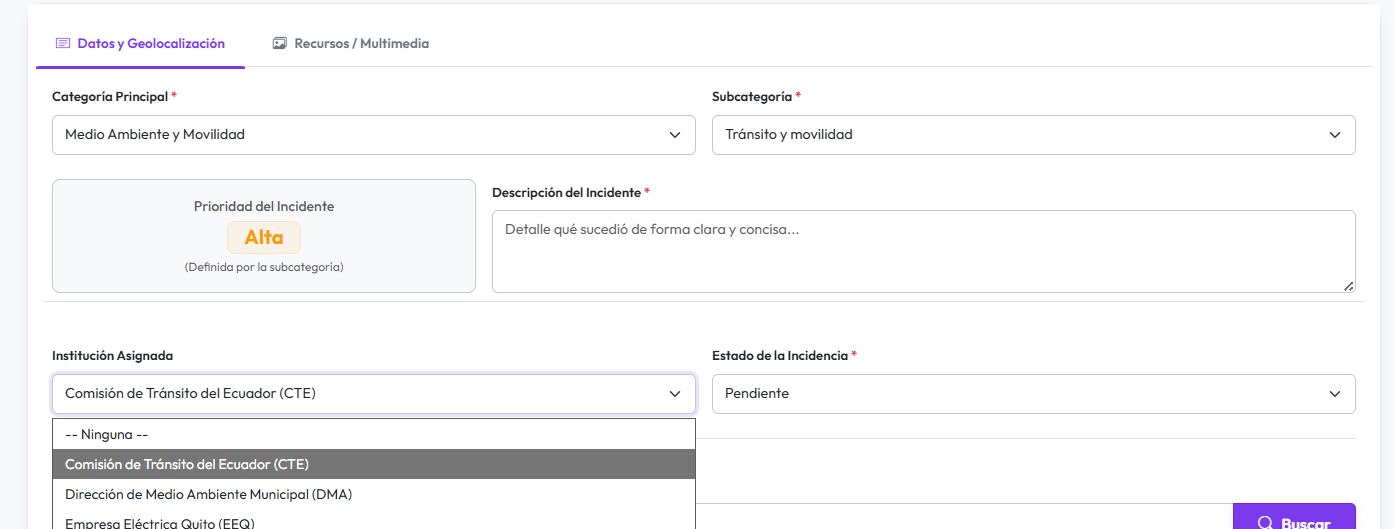
\includegraphics[width=0.9\textwidth]{imagenes/cp-f-06-institucion-asignada.png}
            \caption{Evidencia.}
        \end{figure}
        Sin embargo, siempre y cuando el usuario tenga roles administrativos, tendrá la posibilidad
        de ver el campo de institución y de modificarlo en un caso necesario.
    \end{itemize}

    \item \textbf{CP-F-07} (Agregar comentario) - Fecha: 8/07/2026
    \begin{itemize}
        \item \textbf{Resultado:} [Aprobado]
        \item \textit{Evidencia:}
        
        \begin{figure}[H] % La 'H' mayúscula obliga a la imagen a quedarse EXACTAMENTE aquí
            \centering
            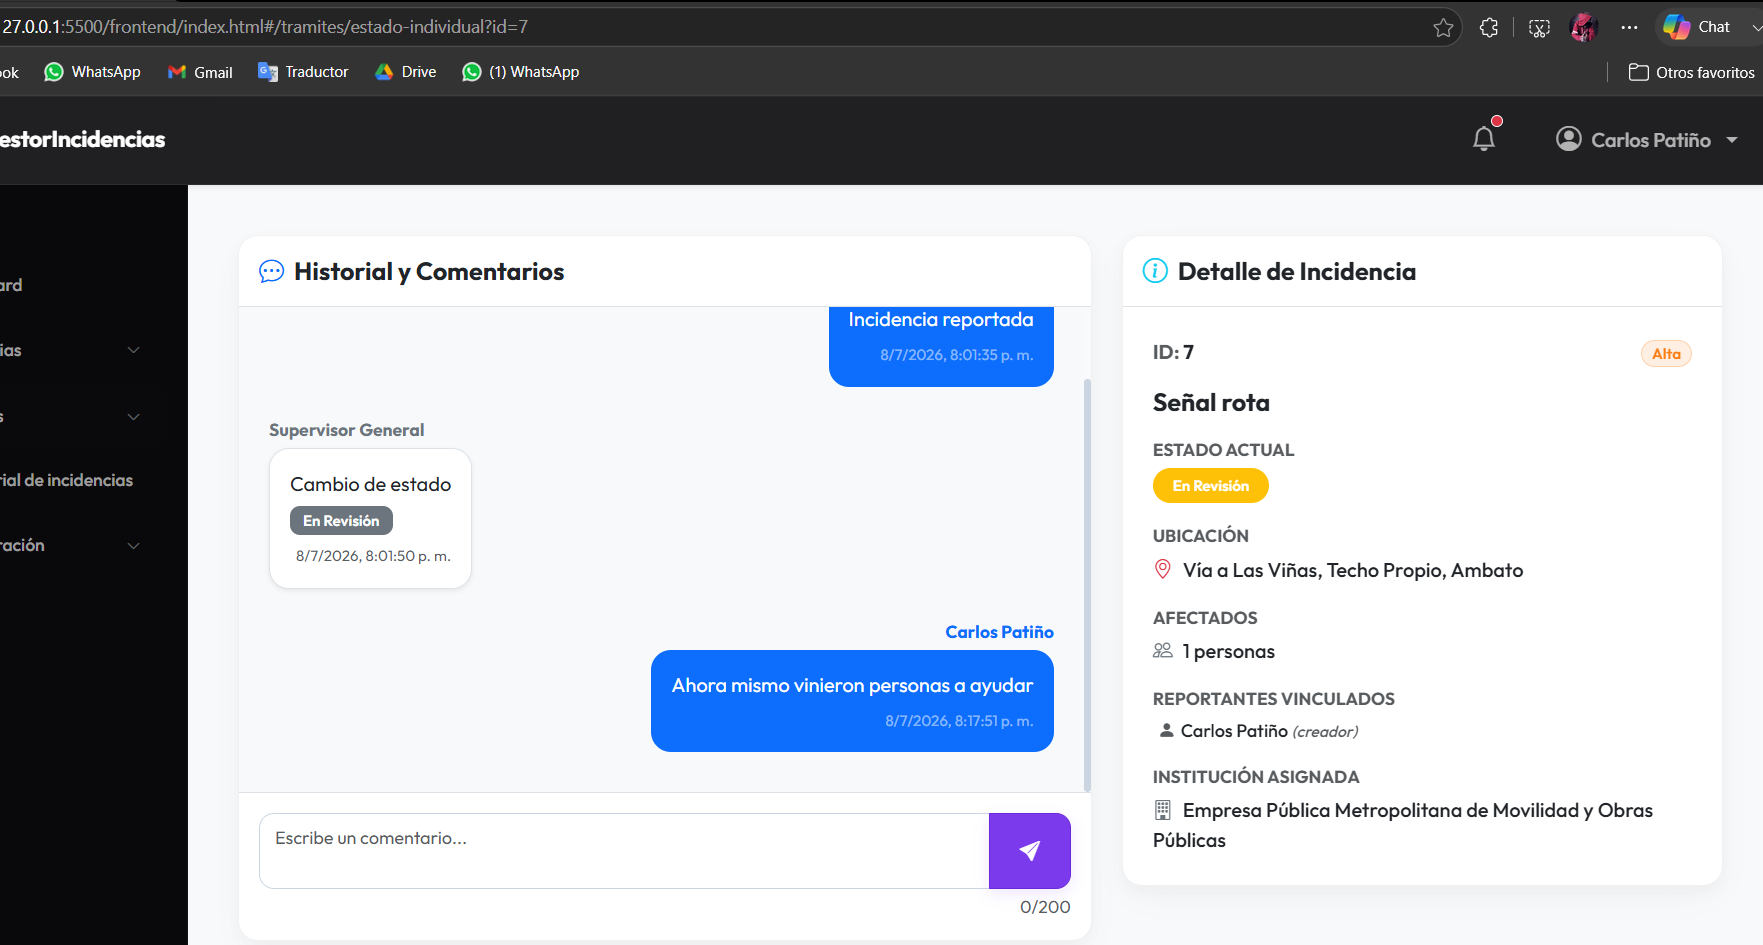
\includegraphics[width=0.9\textwidth]{imagenes/cp-f-07.png}
            \caption{Evidencia.}
        \end{figure}
    \end{itemize}

    \item \textbf{CP-F-08} (Generar notificación) - Fecha: 8/07/2026
    \begin{itemize}
        \item \textbf{Resultado:} [Por implementar]
        \item \textit{Evidencia:}
        
        Esta funcionalidad está pendiente de implementar, se la aplicará en el transcurso de los días posteriores.
    \end{itemize}

    \item \textbf{CP-F-09} (Clasificar prioridad) - Fecha: 7/07/2026
    \begin{itemize}
        \item \textbf{Resultado:} [Aprobado]
        \item \textit{Evidencia:}
        
        \begin{figure}[H] % La 'H' mayúscula obliga a la imagen a quedarse EXACTAMENTE aquí
            \centering
            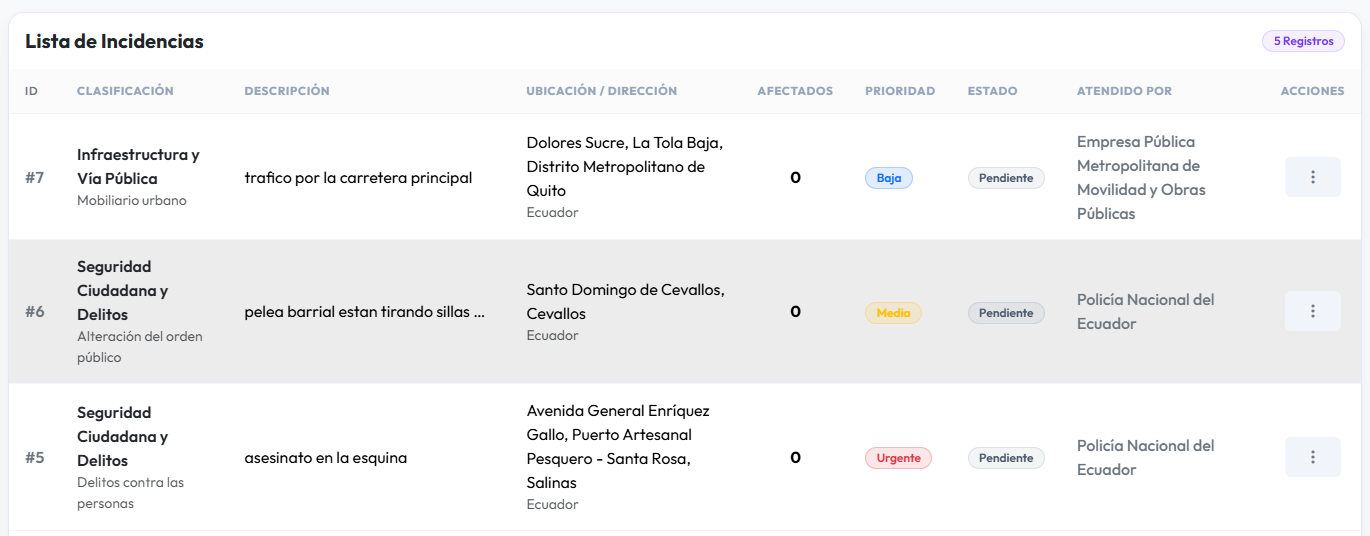
\includegraphics[width=0.9\textwidth]{imagenes/cp-f-09-prioridades.png}
            \caption{Evidencia.}
        \end{figure}
        Se muestra la lista con los estados correctamente jerarquizados por su color
    \end{itemize}

    \item \textbf{CP-F-10} (Asignar tipo/subtipo) - Fecha: 7/07/2026
    \begin{itemize}
        \item \textbf{Resultado:} [Aprobado]
        \item \textit{Evidencia:}
        
        \begin{figure}[H] % La 'H' mayúscula obliga a la imagen a quedarse EXACTAMENTE aquí
            \centering
            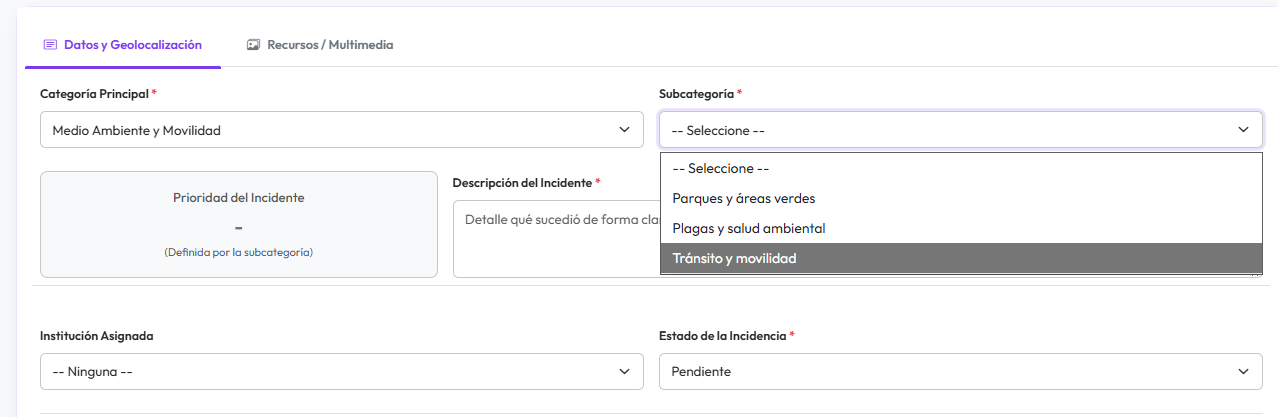
\includegraphics[width=0.9\textwidth]{imagenes/cp-f-06-asignar-subcat-primero.png}
            \caption{Evidencia.}
        \end{figure}
        Al momento de seleccionar una categoría, se cargan las subcategorías relacionadas a esta.

    \end{itemize}

    
    \item \textbf{CP-F-11} (Registrar ubicación) - Fecha: 7/07/2026
    \begin{itemize}
        \item \textbf{Resultado:} [Aprobado]
        \item \textit{Evidencia:}
        
        \begin{figure}[H] % La 'H' mayúscula obliga a la imagen a quedarse EXACTAMENTE aquí
            \centering
            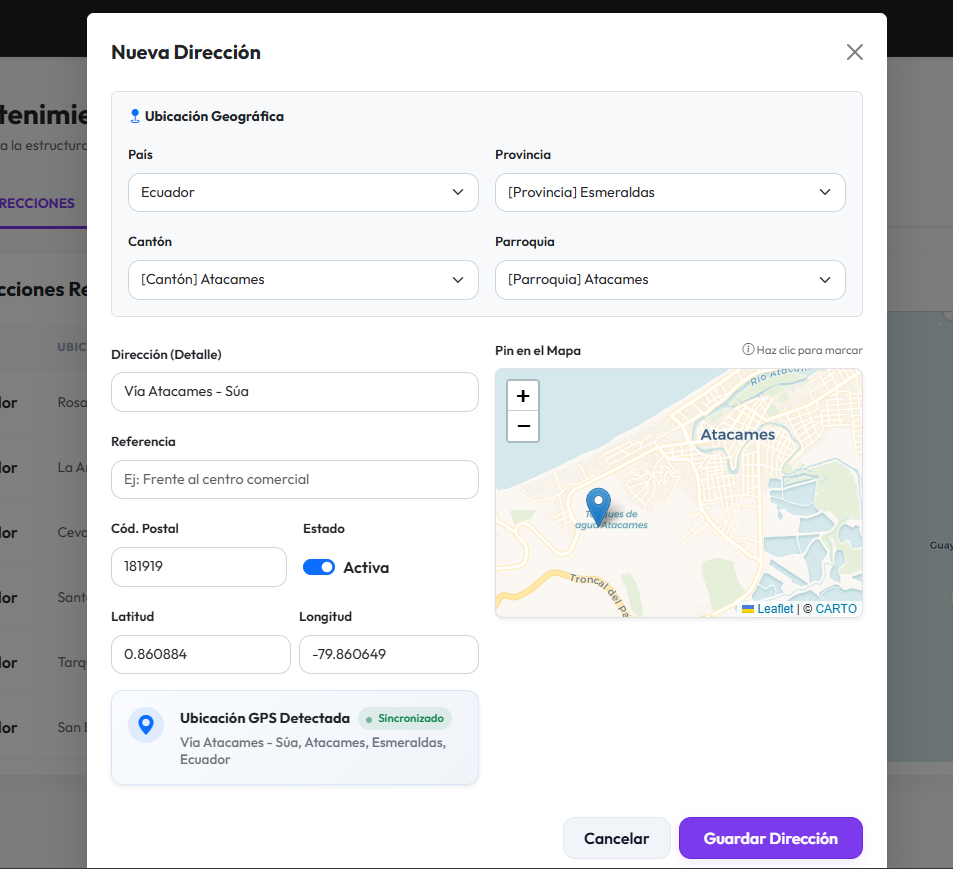
\includegraphics[width=0.9\textwidth]{imagenes/cp-f-11.png}
            \caption{Evidencia.}
        \end{figure}
        Al seleccionar la ubicación en el mapa, se autocompletarán los campos.
        En caso de que el lugar no se ilustre en Leaflet, se le habilita al usuario
        la opción de especificar manualmente la zona.
    \end{itemize}


    \item \textbf{CP-F-12} (Consulta por estado) - Fecha: 8/07/2026
    \begin{itemize}
        \item \textbf{Resultado:} [Por implementar]
        \item \textit{Evidencia:}
        
        La consulta por estados actualmente no está implementada, pero se aplicará un filtro por estado para el historial en caso de que sea necesario.
    \end{itemize}
    \item \textbf{CP-F-13} (Consulta por tipo) - Fecha: 8/07/2026
    \begin{itemize}
        \item \textbf{Resultado:} [Por implementar]
        \item \textit{Evidencia:}
        
        La consulta por tipos actualmente no está implementada, pero se aplicará un filtro por tipo para el historial en caso de que sea necesario.
    \end{itemize}
    \item \textbf{CP-F-14} (Dashboard métricas) - Fecha: 8/07/2026
    \begin{itemize}
        \item \textbf{Resultado:} [Aprobado]
        \item \textit{Evidencia:}
        
        \begin{figure}[H] % La 'H' mayúscula obliga a la imagen a quedarse EXACTAMENTE aquí
            \centering
            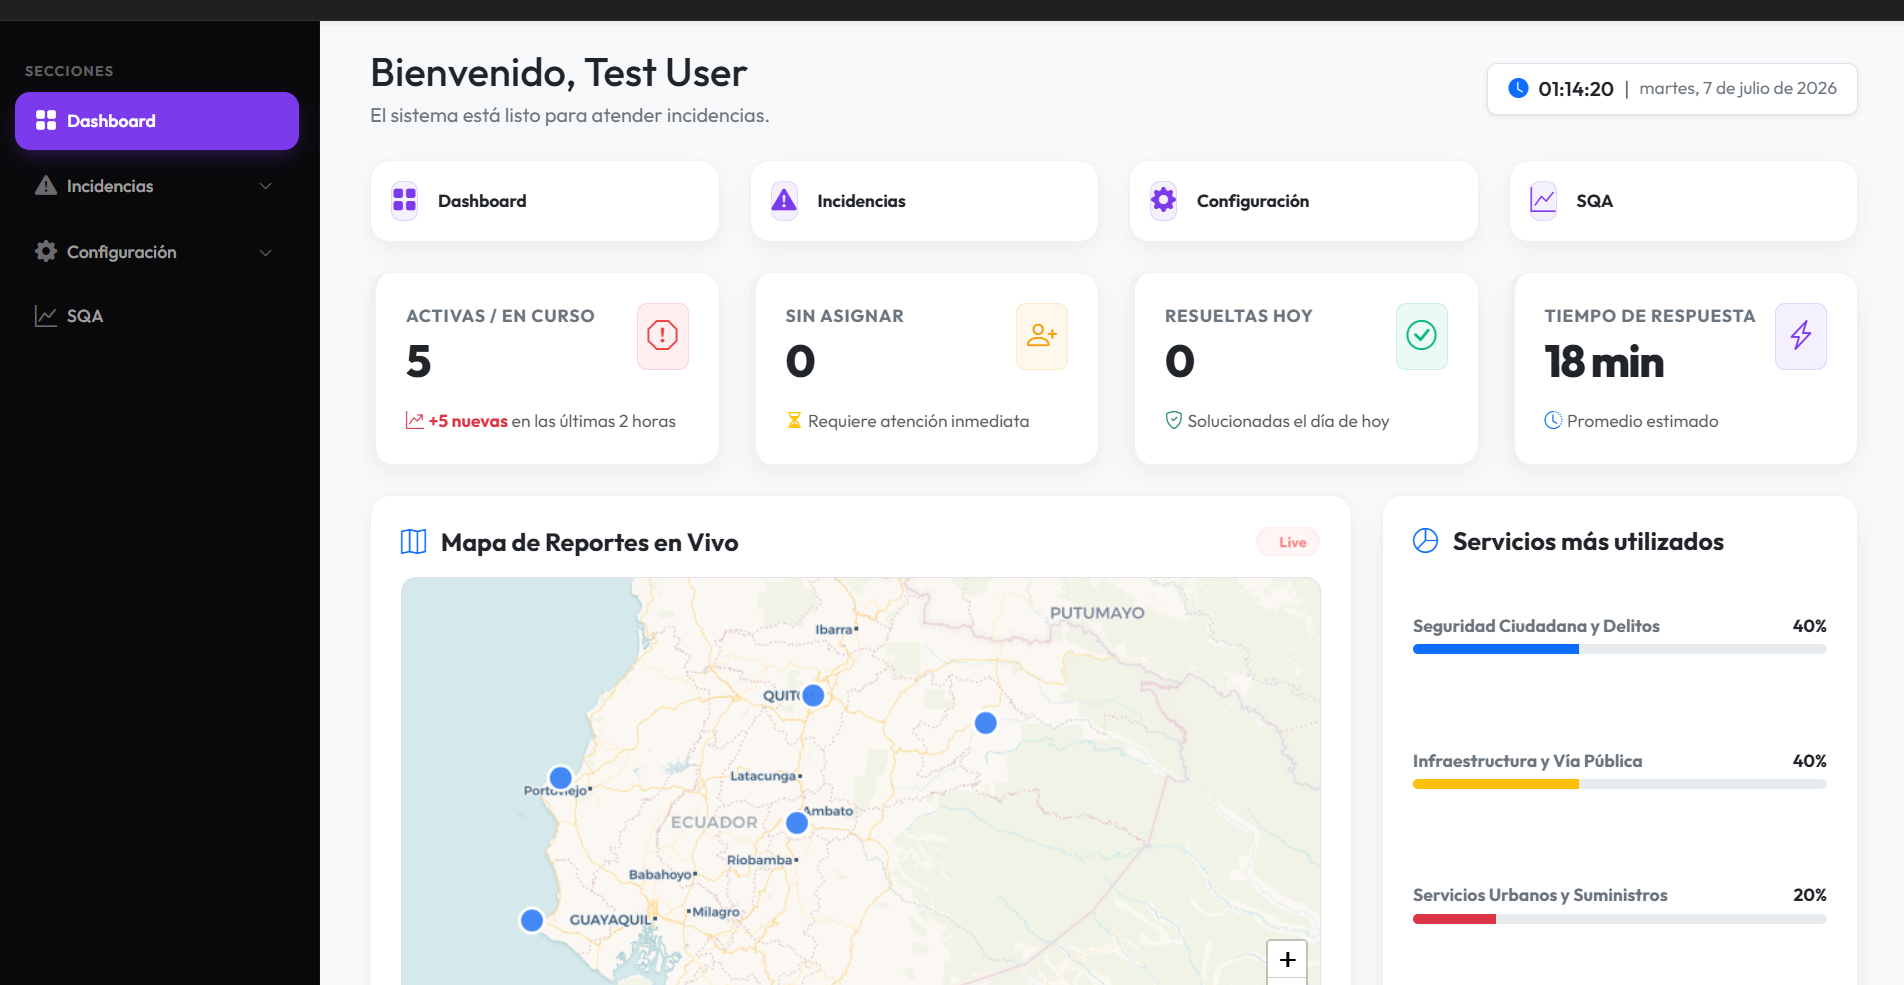
\includegraphics[width=0.9\textwidth]{imagenes/cp-f-14.png}
            \caption{Evidencia.}
        \end{figure}
        Este es el Dashboard principal, aquí se muestran métricas básicas como la cantidad de incidencias registradas a lo largo del tiempo,
        las no asignadas, las resueltas y el tiempo de respuesta promedio calculado dinámicamente.

    \end{itemize}
    \item \textbf{CP-F-15} (Auditoría automática) - Fecha: 8/07/2026
    \begin{itemize}
        \item \textbf{Resultado:} [Aprobado]
        \item \textit{Evidencia:}
        
        \begin{figure}[H] % La 'H' mayúscula obliga a la imagen a quedarse EXACTAMENTE aquí
            \centering
            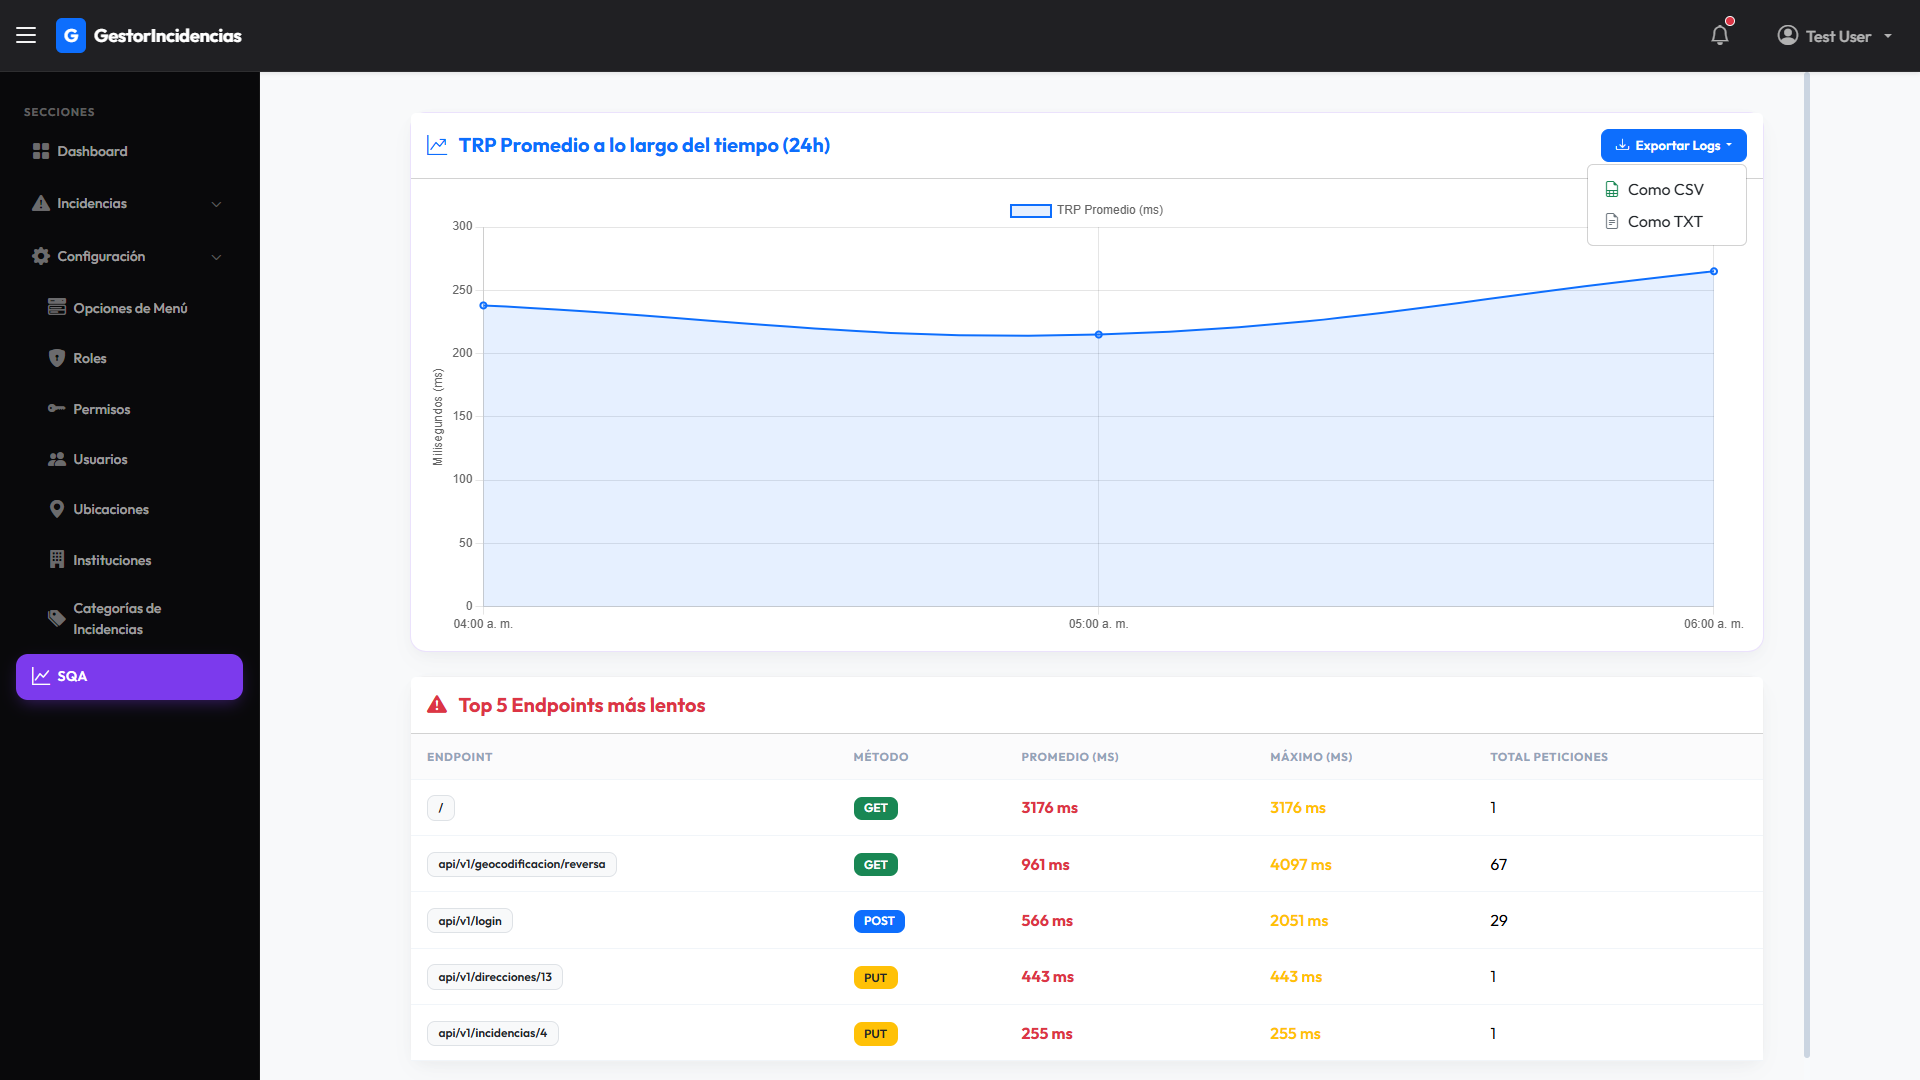
\includegraphics[width=0.9\textwidth]{imagenes/cp-f-15.png}
            \caption{Evidencia.}
        \end{figure}
        Esta pantalla muestra el Tiempo de Respuesta Promedio de las rutas a lo largo del tiempo.
        Las que se hacen notar son las más lentas (con mayor tiempo), reflejadas en la tabla inferior.
        Por debajo se ejecuta un worker que está constantemente calculando el TRP promedio de cada
        consulta REST que se hace.
    \end{itemize}
\end{itemize}

\subsection{Pruebas de Validación}

\begin{itemize}
    \item \textbf{CP-V-01} (Latitud fuera de rango) - Fecha: 7/07/2026
    \begin{itemize}
        \item \textbf{Resultado:} [Aprobado]
        \item \textit{Evidencia:}
        
        \begin{figure}[H] % La 'H' mayúscula obliga a la imagen a quedarse EXACTAMENTE aquí
            \centering
            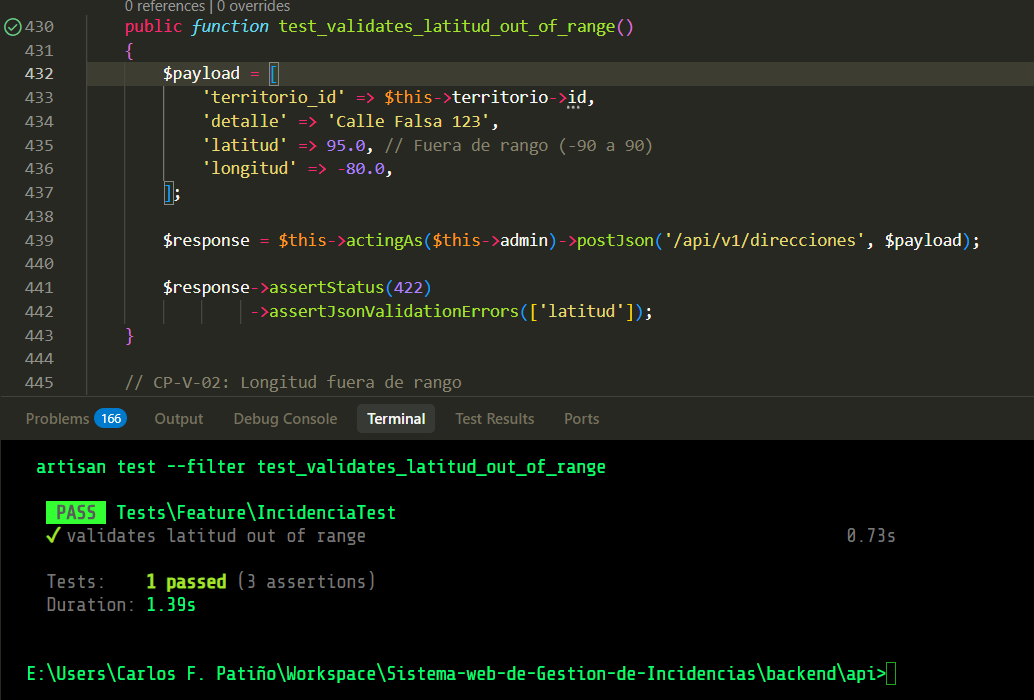
\includegraphics[width=0.9\textwidth]{imagenes/cp-v-01.png}
            \caption{Evidencia.}
        \end{figure}

    \end{itemize}
    \item \textbf{CP-V-02} (Longitud fuera de rango) - Fecha: 7/07/2026
    \begin{itemize}
        \item \textbf{Resultado:} [Aprobado]
        \item \textit{Evidencia:}
        
        \begin{figure}[H] % La 'H' mayúscula obliga a la imagen a quedarse EXACTAMENTE aquí
            \centering
            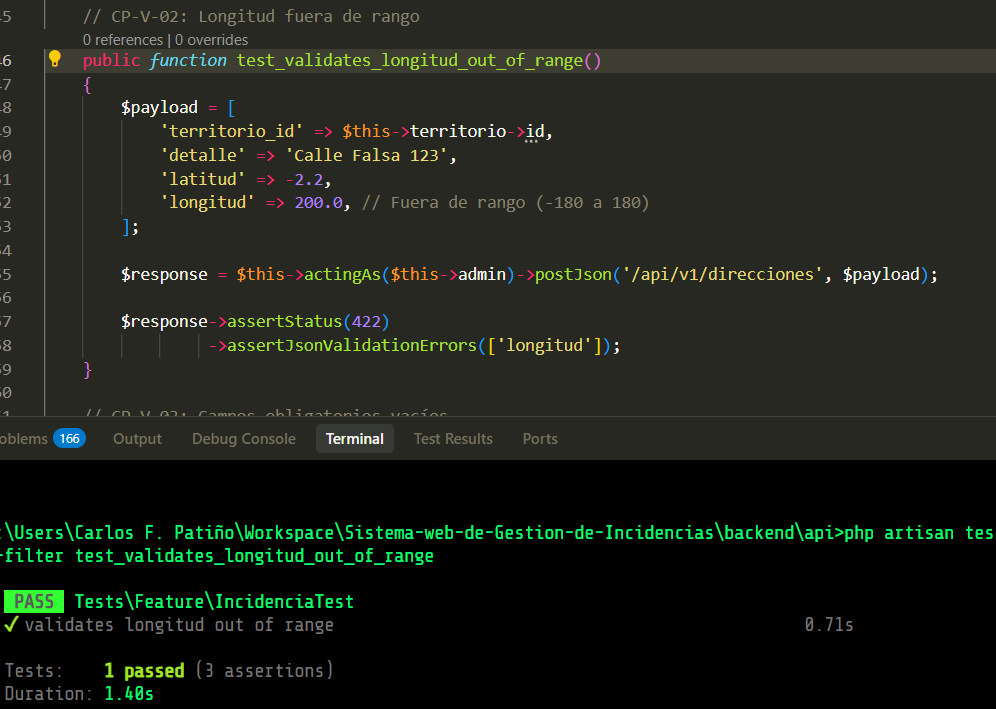
\includegraphics[width=0.9\textwidth]{imagenes/cp-v-02.png}
            \caption{Evidencia.}
        \end{figure}
    \end{itemize}
    \item \textbf{CP-V-03} (Campos obligatorios vacíos) - Fecha: 7/07/2026
    \begin{itemize}
        \item \textbf{Resultado:} [Aprobado]
        \item \textit{Evidencia:}
        
        \begin{figure}[H] % La 'H' mayúscula obliga a la imagen a quedarse EXACTAMENTE aquí
            \centering
            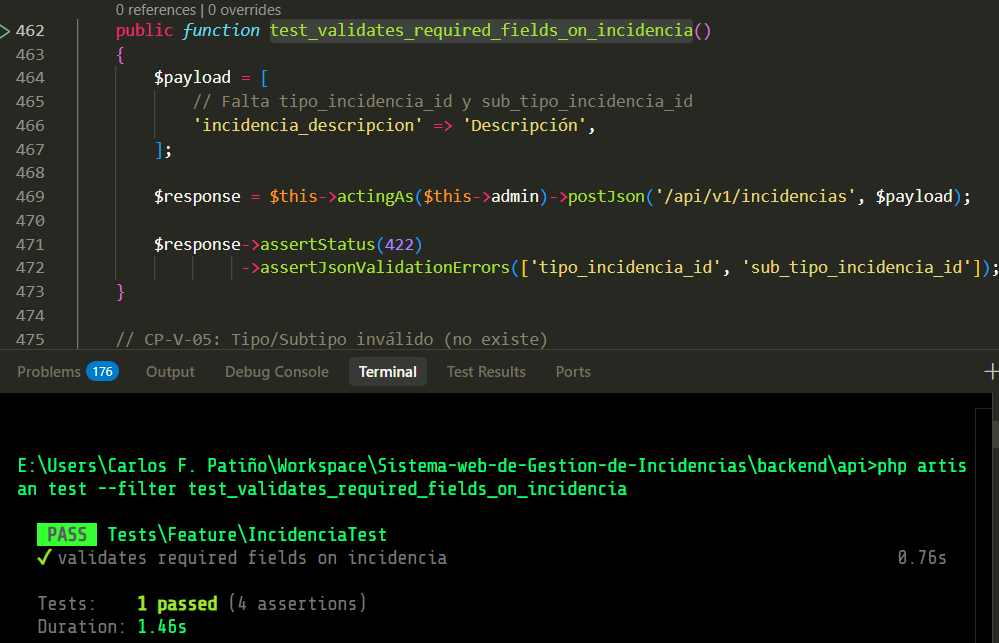
\includegraphics[width=0.9\textwidth]{imagenes/cp-v-03.png}
            \caption{Evidencia.}
        \end{figure}
    \end{itemize}
    \item \textbf{CP-V-04} (Comentario supera longitud) - Fecha: 8/07/2026
    \begin{itemize}
        \item \textbf{Resultado:} [Aprobado]
        \item \textit{Evidencia:}
        
        \begin{figure}[H] % La 'H' mayúscula obliga a la imagen a quedarse EXACTAMENTE aquí
            \centering
            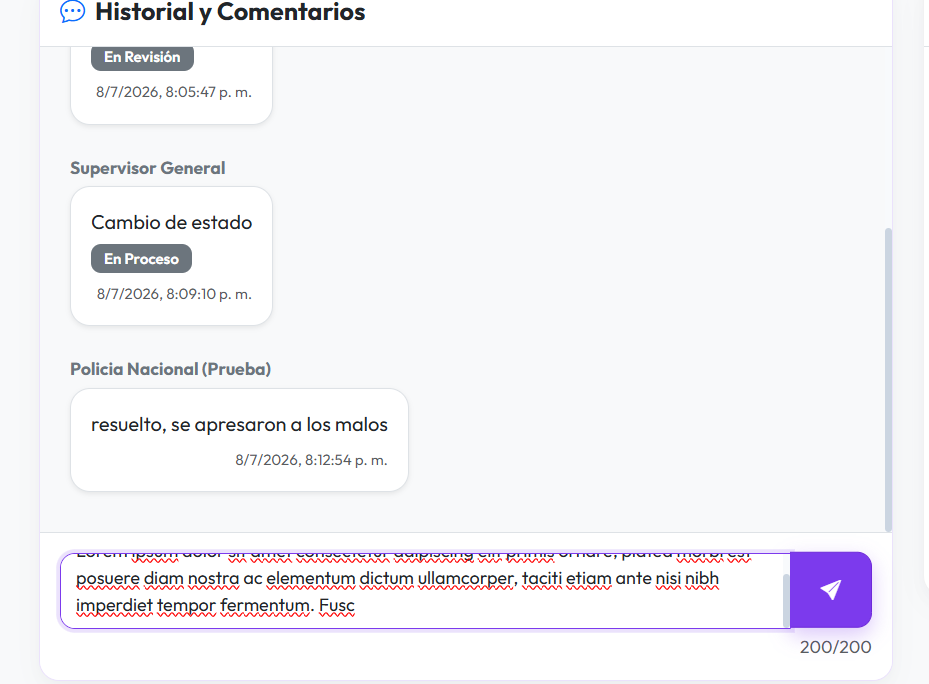
\includegraphics[width=0.9\textwidth]{imagenes/cp-v-04.png}
            \caption{Evidencia.}
        \end{figure}
    \end{itemize}
    \item \textbf{CP-V-05} (Tipo/Subtipo inválido) - Fecha: 7/07/2026
    \begin{itemize}
        \item \textbf{Resultado:} [Aprobado]
        \item \textit{Evidencia:}
        
        \begin{figure}[H] % La 'H' mayúscula obliga a la imagen a quedarse EXACTAMENTE aquí
            \centering
            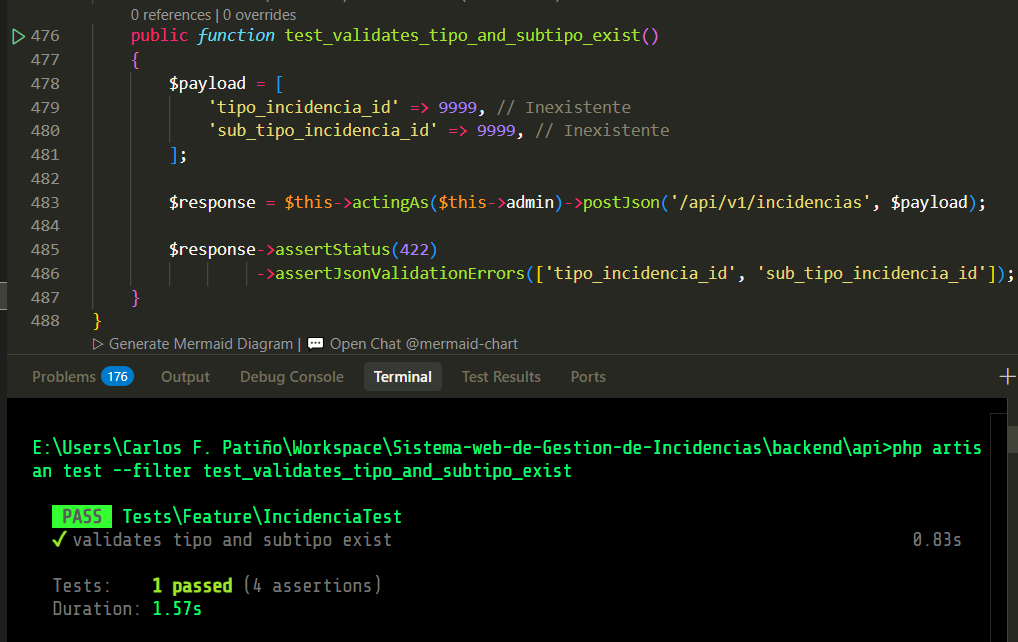
\includegraphics[width=0.9\textwidth]{imagenes/cp-v-05.png}
            \caption{Evidencia.}
        \end{figure}

        Los comentarios están limitados a 200 caracteres para evitar spam y contenido muy extenso
    \end{itemize}
\end{itemize}

\subsection{Pruebas de Seguridad}

\begin{itemize}
    \item \textbf{CP-S-01} (Acceso sin autenticación) - Fecha: 7/07/2026
    \begin{itemize}
        \item \textbf{Resultado:} [Aprobado]
        \item \textit{Evidencia:}
        
        \begin{figure}[H] % La 'H' mayúscula obliga a la imagen a quedarse EXACTAMENTE aquí
            \centering
            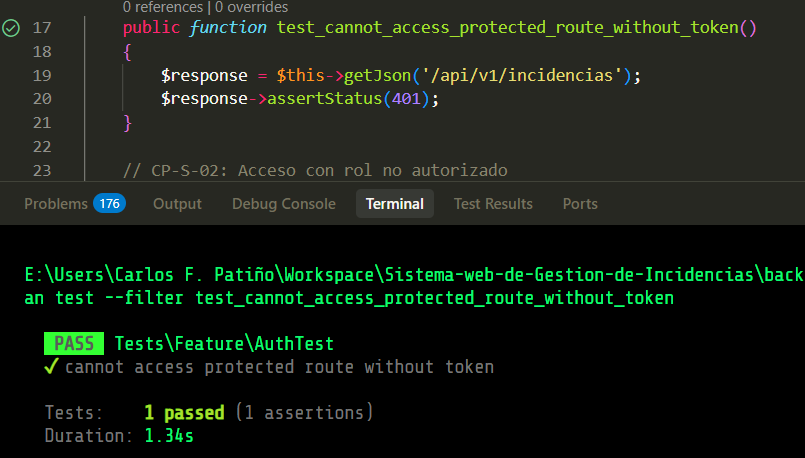
\includegraphics[width=0.9\textwidth]{imagenes/cp-s-01.png}
            \caption{Evidencia.}
        \end{figure}
    \end{itemize}
    \item \textbf{CP-S-02} (Acceso con rol no autorizado) - Fecha: 7/07/2026
    \begin{itemize}
        \item \textbf{Resultado:} [Aprobado]
        \item \textit{Evidencia:}
        
        \begin{figure}[H] % La 'H' mayúscula obliga a la imagen a quedarse EXACTAMENTE aquí
            \centering
            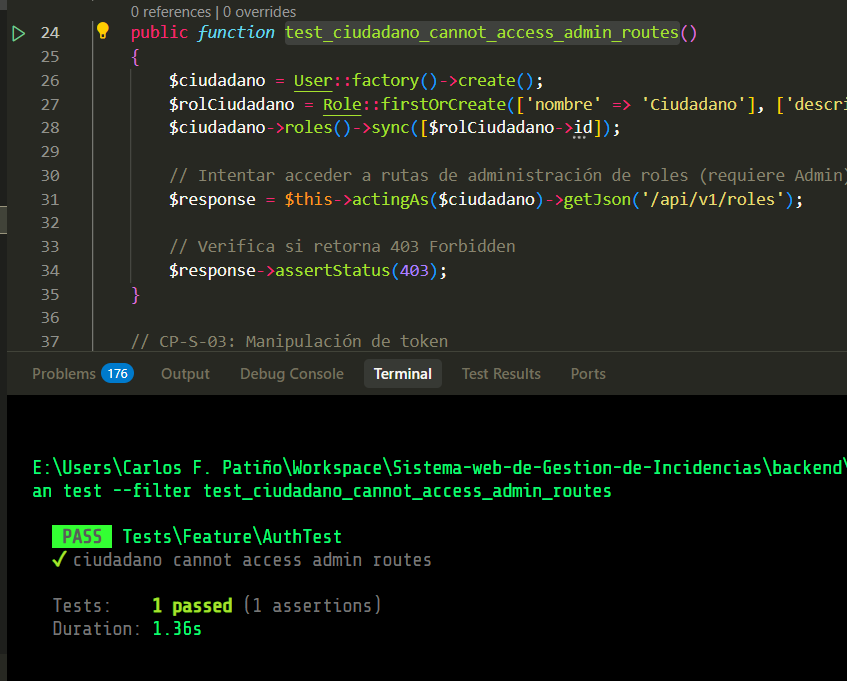
\includegraphics[width=0.9\textwidth]{imagenes/cp-s-02.png}
            \caption{Evidencia.}
        \end{figure}
    \end{itemize}
    \item \textbf{CP-S-03} (Manipulación de token) - Fecha: 7/07/2026
    \begin{itemize}
        \item \textbf{Resultado:} [Aprobado]
        \item \textit{Evidencia:}
        
        \begin{figure}[H] % La 'H' mayúscula obliga a la imagen a quedarse EXACTAMENTE aquí
            \centering
            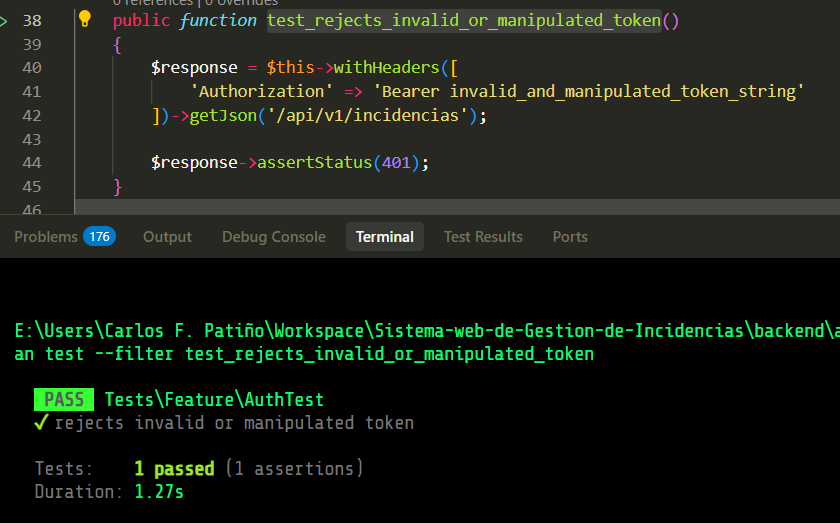
\includegraphics[width=0.9\textwidth]{imagenes/cp-s-03.png}
            \caption{Evidencia.}
        \end{figure}
    \end{itemize}
    \item \textbf{CP-S-04} (Expiración de sesión) - Fecha: 7/07/2026
    \begin{itemize}
        \item \textbf{Resultado:} [Aprobado]
        \item \textit{Evidencia:}
        
        \begin{figure}[H] % La 'H' mayúscula obliga a la imagen a quedarse EXACTAMENTE aquí
            \centering
            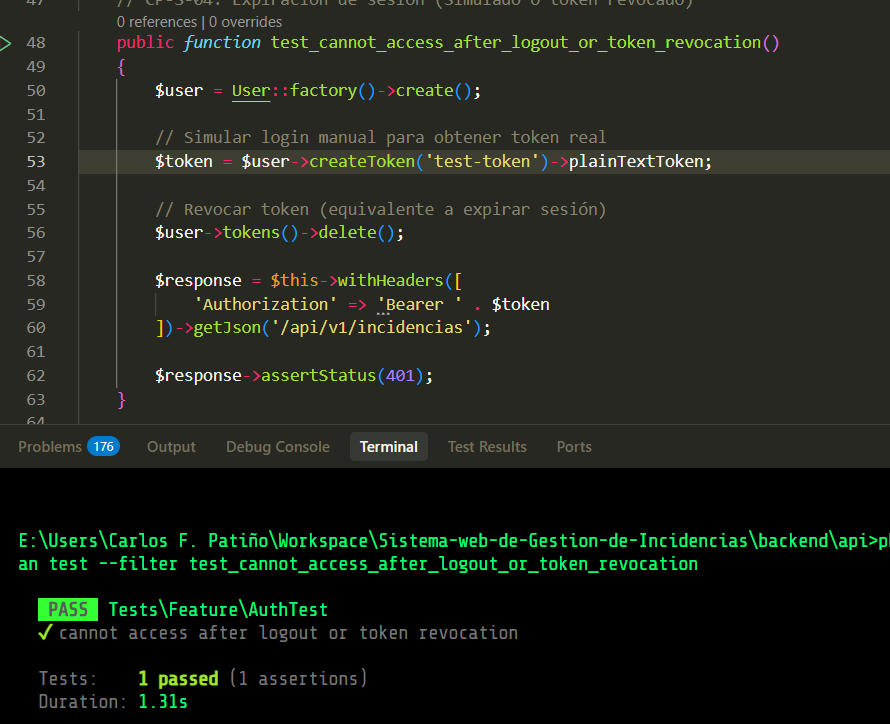
\includegraphics[width=0.9\textwidth]{imagenes/cp-s-04.png}
            \caption{Evidencia.}
        \end{figure}
    \end{itemize}
    \item \textbf{CP-S-05} (Ocultamiento de opciones menú) - Fecha: 7/07/2026
    \begin{itemize}
        \item \textbf{Resultado:} [Aprobado]
        \item \textit{Evidencia:}
        
        \begin{figure}[H] % La 'H' mayúscula obliga a la imagen a quedarse EXACTAMENTE aquí
            \centering
            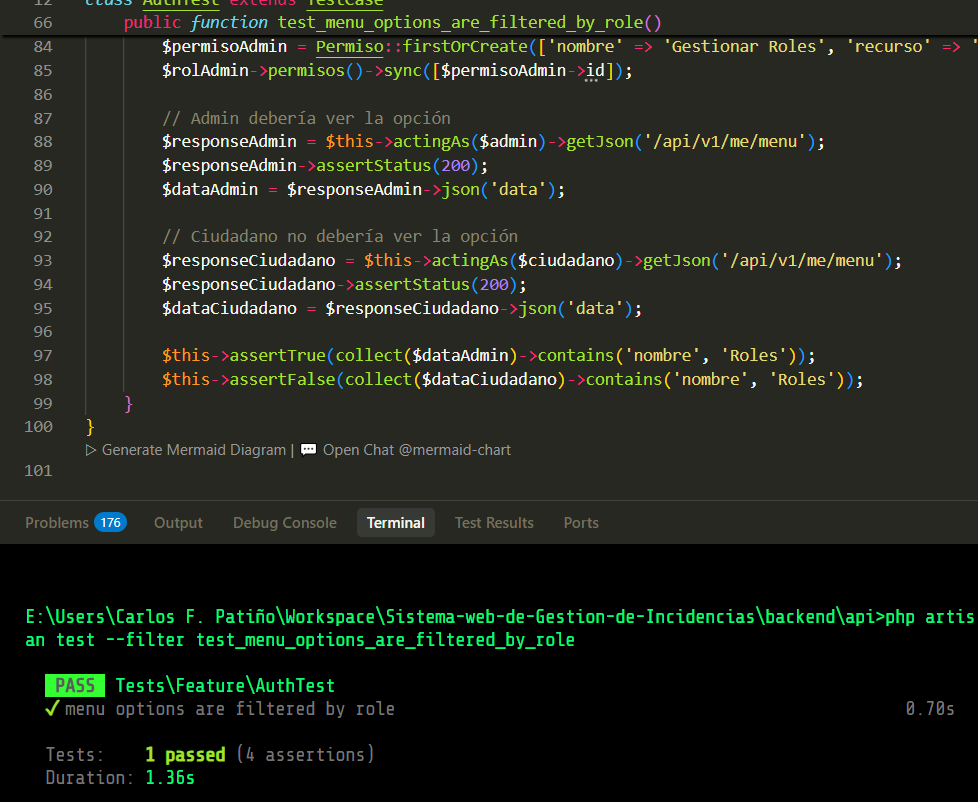
\includegraphics[width=0.9\textwidth]{imagenes/cp-s-05.png}
            \caption{Evidencia.}
        \end{figure}
    \end{itemize}
\end{itemize}
